\section{Análise Exploratória de Dados}
\label{sec:eda}

\subsection{Estratégia Metodológica e Ferramentas Utilizadas}

A análise exploratória de dados conduzida foi concebida como uma investigação sistemática e progressiva, estruturada em torno de um princípio metodológico central: partir da caracterização temporal global da série de alarmes para, gradualmente, decompor o comportamento do sistema em suas dimensões operacionais constituintes --- máquina, turno de produção e correlação com variáveis exógenas. Essa progressão geral para especificação reflete a hierarquia natural dos fenômenos investigados, na qual padrões macrotemporais, como sazonalidades e tendências, precisam ser identificados e isolados antes que comportamentos de máquinas individuais possam ser devidamente interpretados sem confusão.

O ponto de partida foi a transformação do dado bruto em representação analítica adequada. O \textit{dataset} original consiste em eventos discretos de alarme --- registros individuais --- que, por sua natureza pontual, não são diretamente compatíveis com os métodos de análise de séries temporais contínuas. A solução adotada foi a agregação diária dos eventos por volume global, produzindo uma série temporal de contagens com granularidade de um dia. Essa representação foi empregada no diagnóstico de hiatos, na análise espectral, na decomposição aditiva, na autocorrelação e na associação com variáveis exógenas. As análises que dependem da identidade da máquina, do horário ou da ordem exata dos eventos --- sazonalidade intradiária, IAT e recorrência --- utilizaram os registros tratados em granularidade original, sem reconstrução de uma segunda base.

Todo o desenvolvimento analítico foi realizado em Python 3.13, em arquivos de código modular combinado com \textit{notebooks Jupyter}, oferecendo a combinação de executabilidade limpa e documentação narrativa que garantem boa reprodutibilidade. O código completo, organizado em módulos correspondentes a cada etapa da análise, encontra-se disponível em repositório público no GitHub~\cite{gpam_manufacturing_alarms}, conferindo transparência e rastreabilidade metodológica de trabalho.

As bibliotecas computacionais utilizadas foram selecionadas com base em adoção consolidada na comunidade científica e adequação às tarefas específicas de cada etapa da análise. A biblioteca \textit{Pandas} constituiu a estrutura central de manipulação e indexação temporal dos dados, por sua capacidade nativa de operar com índices de data e hora e realizar reestruturações e agregações temporais de forma eficiente; operações numéricas auxiliares foram realizadas com \textit{NumPy}; a análise espectral foi implementada com os módulos \texttt{scipy.fft} e \texttt{scipy.signal} da biblioteca \textit{SciPy}; os coeficientes de correlação de Spearman foram obtidos com \texttt{scipy.stats}; e as funções de autocorrelação e autocorrelação parcial foram computadas com \textit{Statsmodels}. A decomposição utilizada no resultado final foi implementada de forma modular no próprio projeto, mediante média móvel centrada de 30 dias e estimação sequencial das componentes semanal e mensal. As visualizações foram produzidas com Matplotlib e Seaborn.

A adoção de uma pilha computacional inteiramente baseada em software livre e de código aberto assegura que os resultados obtidos sejam integralmente reproduzíveis por pesquisadores externos sem dependência de licenças proprietárias, alinhando-se aos princípios de ciência aberta e replicabilidade metodológica~\cite{araujo2025cienciaaberta}.

\subsection{Pré-Processamento e Agregação Temporal}

O \textit{dataset} bruto, composto por eventos discretos de alarme com carimbo de tempo individual, foi transformado em uma série temporal contínua apta à análise estatística por meio de um \textit{pipeline} de pré-processamento implementado em Pandas.

A etapa inicial compreendeu a padronização dos nomes e tipos de dados --- com conversão explícita do campo \textit{Timestamp} para o formato temporal do Pandas ---, a remoção de três registros duplicados, a eliminação de valores ausentes remanescentes e a ordenação cronológica. A agregação foi realizada na granularidade diária por reamostragem do índice temporal, contabilizando o volume global de alarmes. Em seguida, o índice foi expandido para cobrir continuamente o intervalo de 11 de janeiro de 2020 a 16 de maio de 2025, com preenchimento por zero nos dias sem registros, tornando os hiatos explicitamente representados na série.

O resultado é uma série temporal diária bruta com 1.953 observações, das quais 1.528 possuem ao menos um evento e 425 apresentam contagem zero. Uma segunda versão foi construída pela identificação anual de outliers mediante a regra do intervalo interquartil e sua substituição por interpolação linear, complementada nas bordas por preenchimento com o valor válido mais próximo. Ao todo, 106 observações foram tratadas, e a série resultante não contém valores ausentes nem ultrapassa aproximadamente 150 alarmes por dia. A série bruta permaneceu preservada como referência; sazonalidade diária, FFT, decomposição aditiva e autocorrelação foram comparadas nas versões com e sem outliers.

A Figura~\ref{fig:daily-series-comparison} evidencia o efeito desse tratamento. A série sem outliers preserva as mudanças de nível e os períodos sem registros, mas reduz os picos isolados que dominavam a escala da série bruta.

\begin{figure}[H]
    \centering
    \begin{subfigure}{0.45\linewidth}
        \centering
        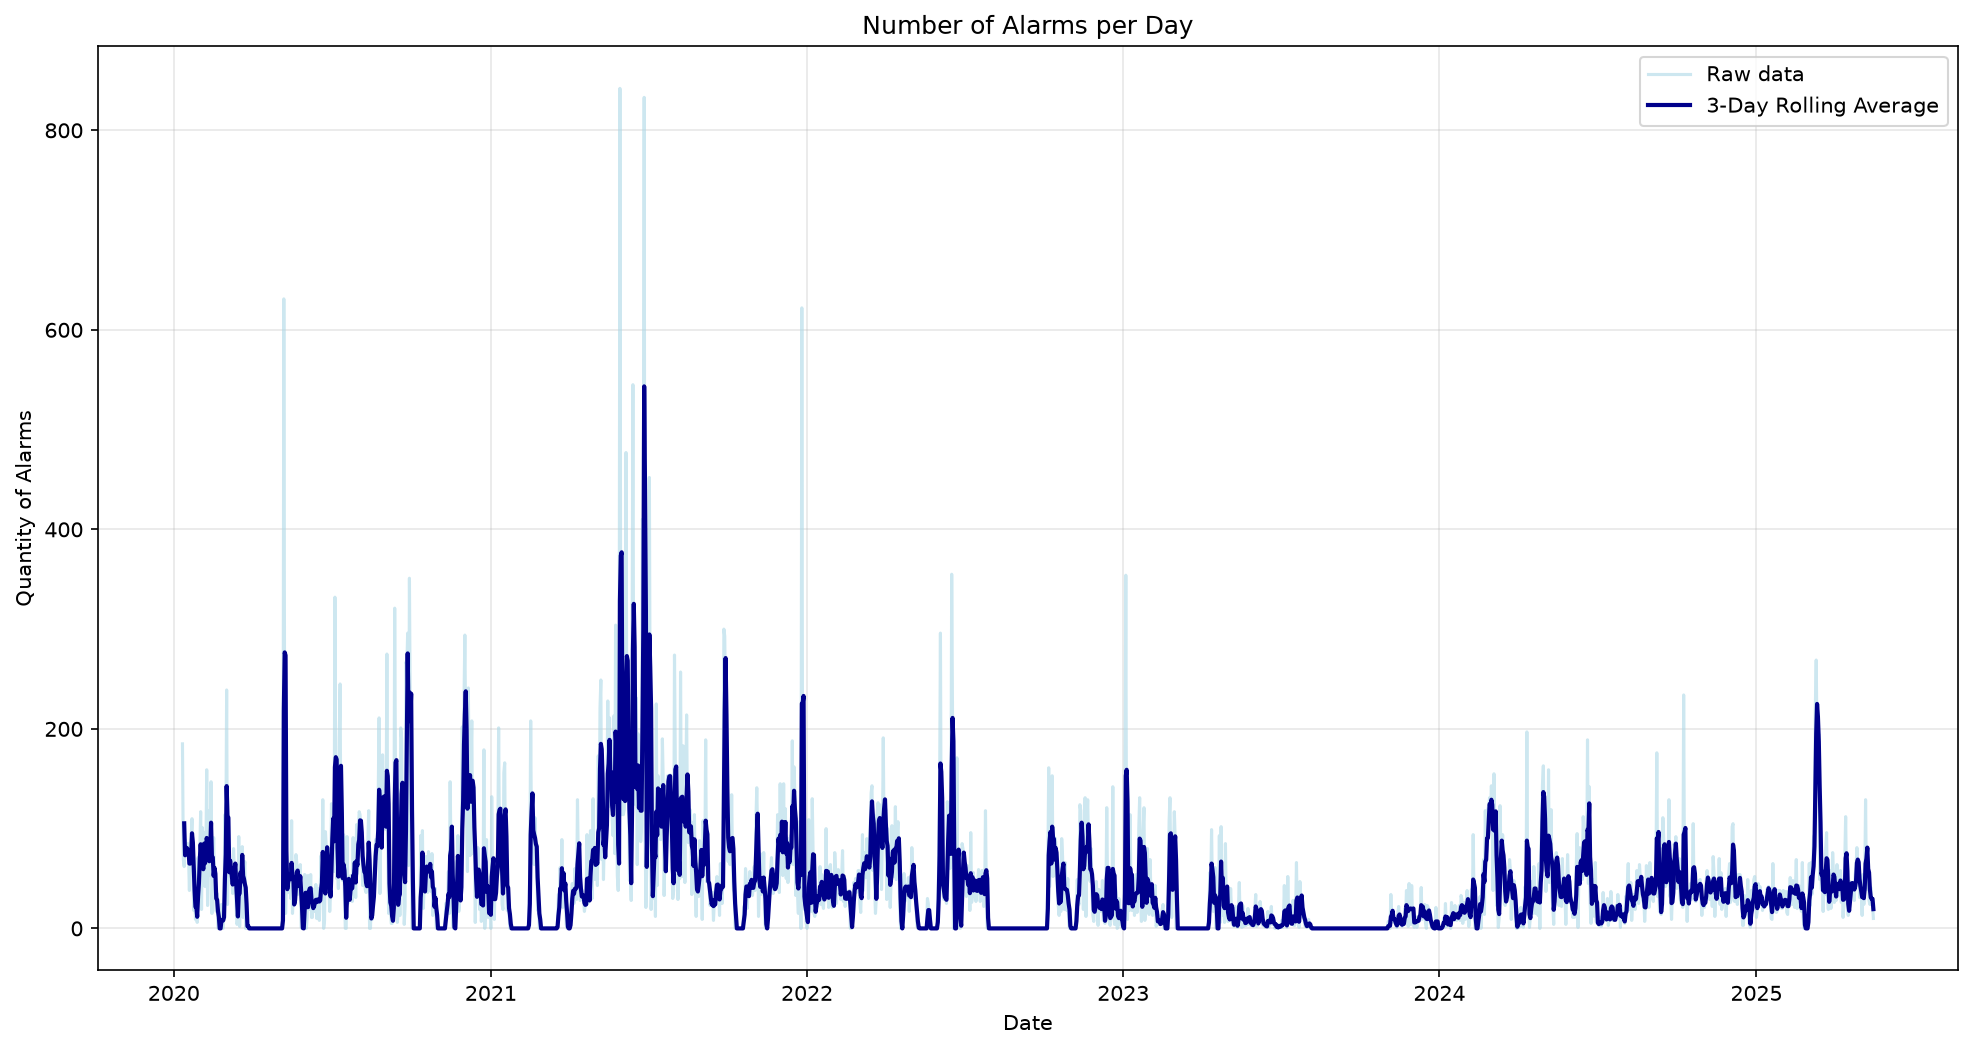
\includegraphics[width=0.6\linewidth]{daily_agg_raw_time_series.png}
        \caption{Série diária bruta.}
        \label{fig:daily-series-raw}
    \end{subfigure}
    \hfill
    \begin{subfigure}{0.45\linewidth}
        \centering
        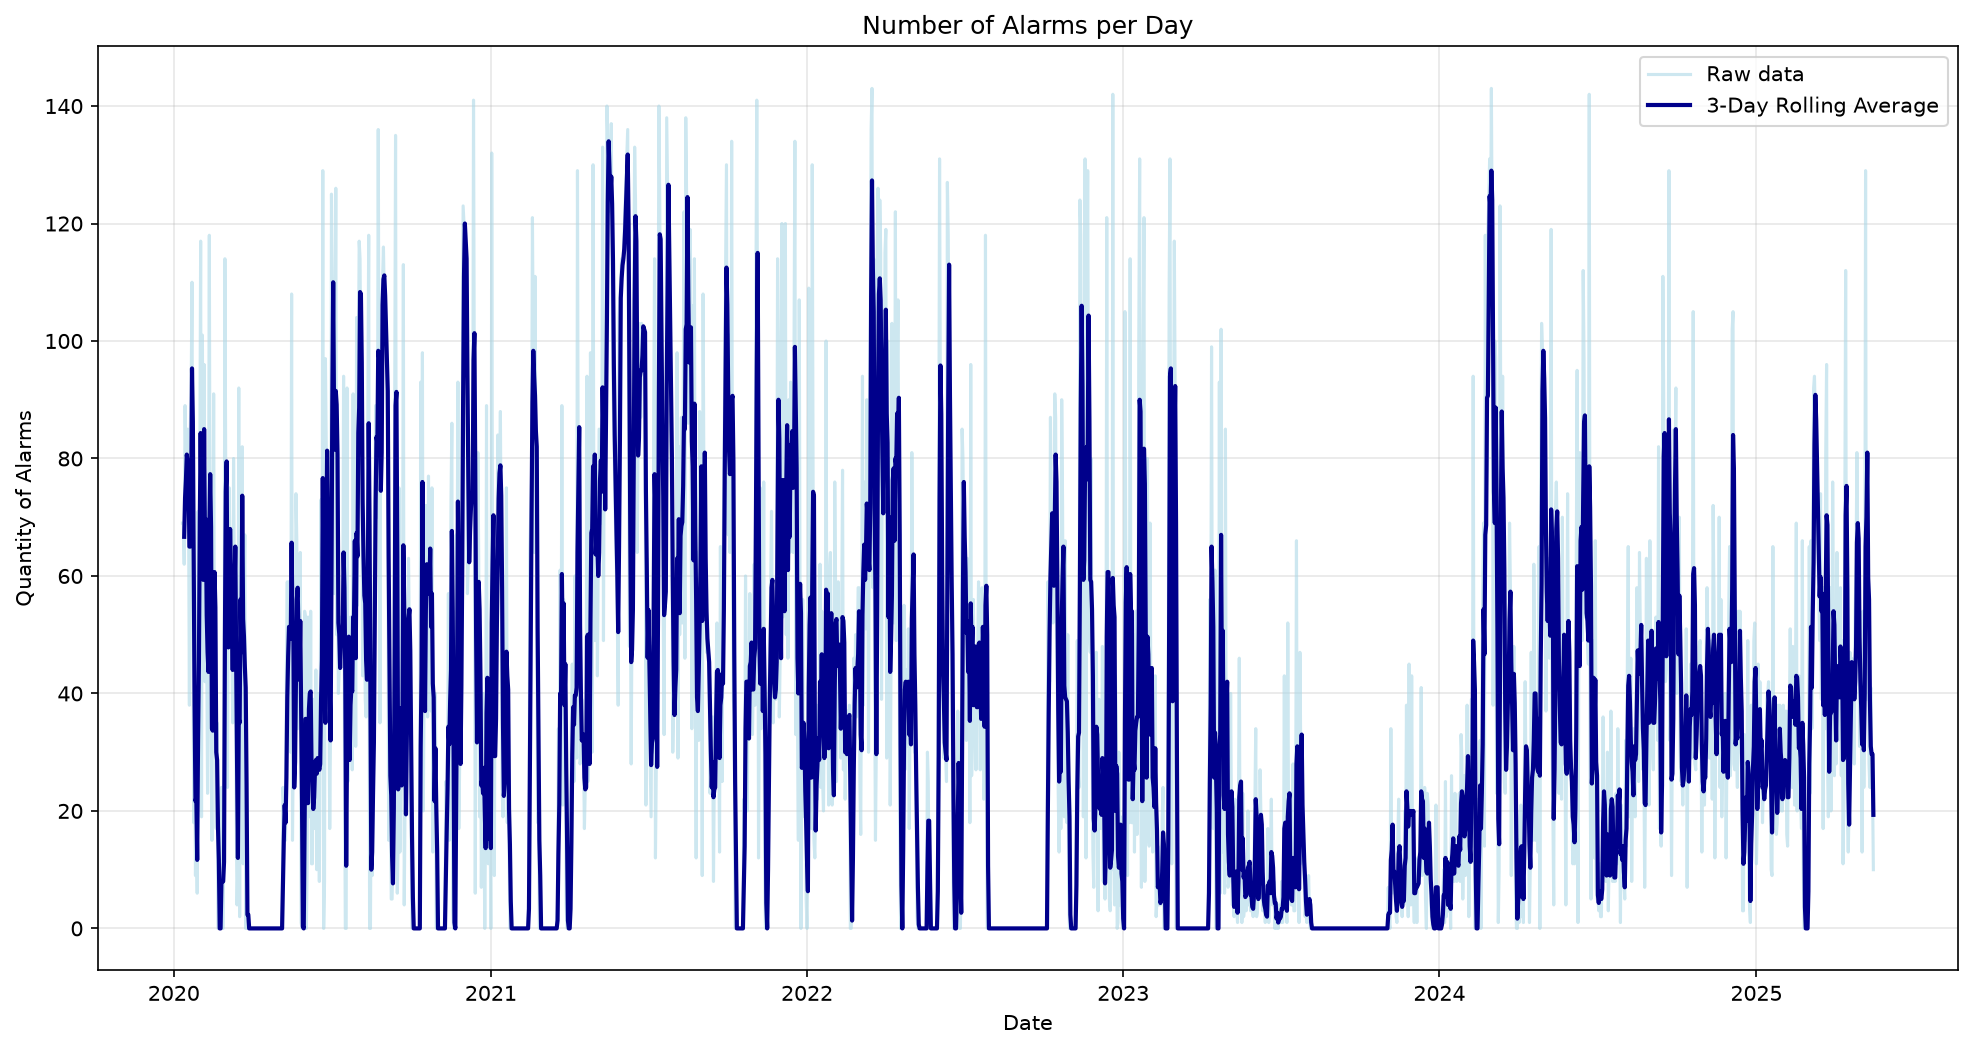
\includegraphics[width=0.6\linewidth]{daily_agg_raw_ts_no_outliers.png}
        \caption{Série diária após o tratamento dos outliers.}
        \label{fig:daily-series-clean}
    \end{subfigure}
    \caption{Volume diário de alarmes antes e depois do tratamento anual de outliers. A comparação preserva o mesmo período e torna visível a redução dos valores extremos.}
    \label{fig:daily-series-comparison}
\end{figure}

\subsection{Diagnóstico e Classificação de Hiatos Temporais}

A presença de períodos de zero alarme na série temporal agregada constitui um desafio metodológico relevante: hiatos introduzem descontinuidades que podem distorcer estimativas de sazonalidade, inflar medidas de autocorrelação e comprometer a validade de modelos treinados sob premissa de continuidade temporal. O diagnóstico sistemático desses períodos foi, portanto, conduzido antes das análises espectral e de correlação.

A identificação foi realizada pela detecção de todas as sequências contíguas de dias com contagem zero na série reindexada. O inventário completo reúne 48 sequências; para a análise de relevância operacional, adotou-se o limiar mínimo de dois dias consecutivos, resultando em 32 hiatos. Essa distinção preserva os episódios de um dia para rastreabilidade, mas impede que ausências isoladas recebam o mesmo peso analítico de paralisações prolongadas.

Os 32 hiatos com pelo menos dois dias foram classificados a partir de intervalos de datas previamente anotados: um período de 41 dias associado à paralisação da COVID-19; três paradas de planta, que totalizam 81 dias; três recessos de Carnaval; quatro intervalos associados à Semana Santa; 19 hiatos sem classificação específica; e dois episódios não resolvidos de 70 e 90 dias, que somam 160 dias. Estes últimos ocorreram entre julho e outubro de 2022 e entre agosto e novembro de 2023 e requerem validação da empresa parceira antes que lhes seja atribuída causa operacional. Nas estimativas de FFT e decomposição, os dias de contagem zero foram tratados como ausentes e interpolados apenas na série de trabalho, mantendo-se os valores originais inalterados na base. Esse procedimento reduz a influência espectral das paralisações sem eliminar a informação de que elas ocorreram.

A distribuição temporal e a classificação dos hiatos são apresentadas na Figura~\ref{fig:classified-gaps}. A visualização destaca tanto as interrupções associadas a eventos conhecidos quanto os dois intervalos extensos cuja causa permanece não validada.

\begin{figure}[H]
    \centering
    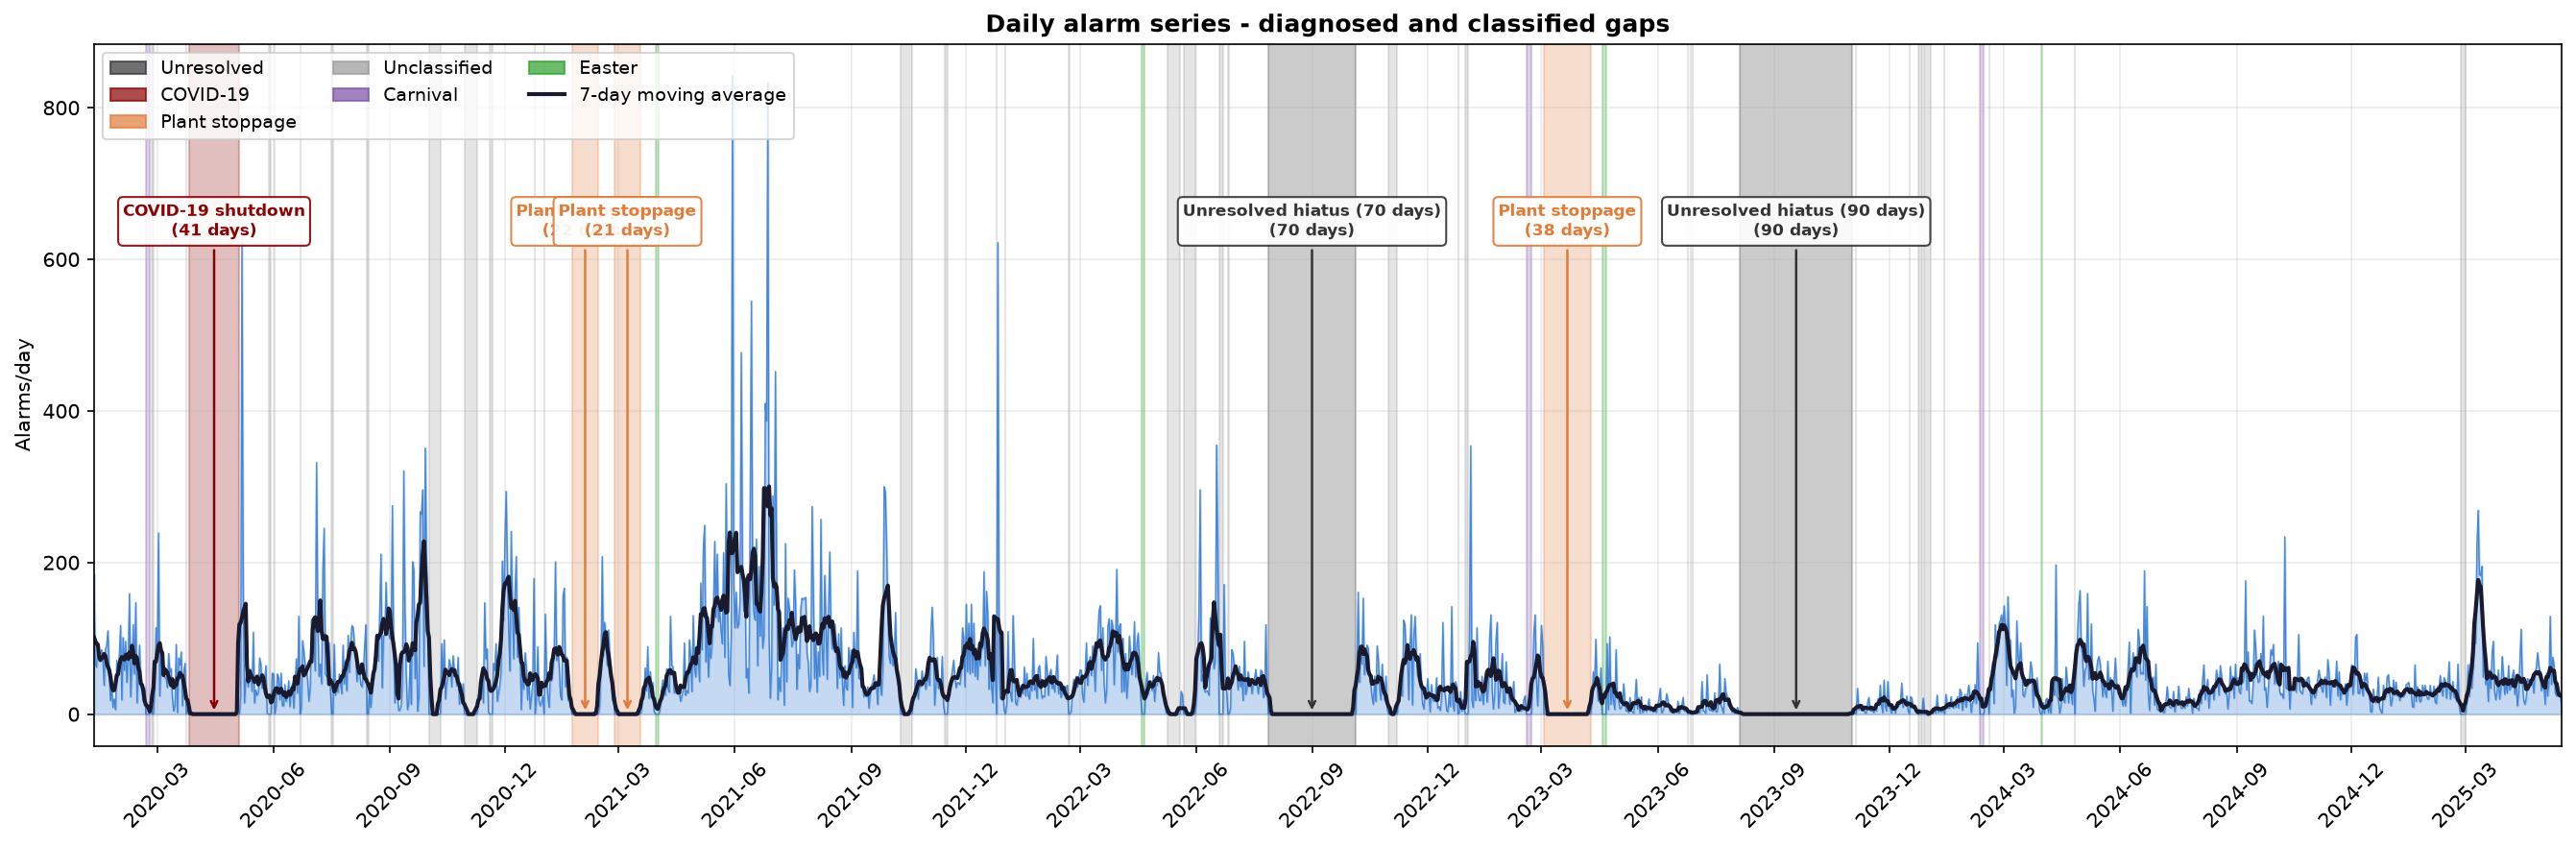
\includegraphics[width=0.7\linewidth]{classified_gap_series_raw.png}
    \caption{Série diária bruta com identificação e classificação dos hiatos temporais. Os intervalos sem alarmes são diferenciados conforme a causa conhecida ou a ausência de classificação validada.}
    \label{fig:classified-gaps}
\end{figure}

\subsection{Análise de Recorrência por Máquina e Turno}

A recorrência foi investigada por meio do IAT (\textit{inter-alarm time}), definido como o intervalo, em minutos, entre um alarme e o evento imediatamente anterior da mesma máquina. Para seu cálculo, os 88.411 registros tratados foram ordenados por máquina e instante de ocorrência, e aplicou-se a diferença temporal dentro de cada grupo. O primeiro evento de cada máquina não possui observação anterior e, portanto, não gera IAT; intervalos nulos ou negativos seriam igualmente desconsiderados. O procedimento produziu 88.391 intervalos positivos válidos para as 20 máquinas.

A distribuição do IAT é fortemente assimétrica à direita, com médias muito superiores às medianas em razão das paralisações e dos grandes hiatos. Por esse motivo, a mediana é a medida mais adequada para comparar a frequência típica entre máquinas. TR19 apresentou o menor IAT mediano, 38,71 minutos, seguida por TR10, com 43,77 minutos, e TR17, com 73,08 minutos. Esses resultados diferenciam TR19 do simples ranking por volume: apesar de registrar 4.957 alarmes, abaixo de TR10 e TR17, ela concentra eventos em intervalos particularmente curtos.

Foram avaliados limiares de 15, 30 e 60 minutos. Em todas as máquinas, ao menos cerca de 25\% dos alarmes pertencem a recorrências inferiores a 15 minutos; no limiar de 60 minutos, a proporção mínima supera aproximadamente 35\%. O limiar intermediário de 30 minutos oferece equilíbrio entre sensibilidade a repetições rápidas e abrangência operacional, razão pela qual foi escolhido para a definição da variável-alvo. Nesse limiar, TR19 apresentou 2.389 recorrências em 4.957 alarmes (48,19\%), TR10 apresentou 3.036 em 6.379 (47,59\%) e TR17 apresentou 2.146 em 5.527 (38,83\%). Na extremidade inferior, TR14 e TR18 registraram 29,92\%, ainda evidenciando que a repetição rápida não se restringe a poucas máquinas.

Para a análise por turno, cada evento foi associado a uma das três janelas de oito horas: primeiro turno, das 6h às 14h; segundo turno, das 14h às 22h; e terceiro turno, das 22h às 6h. Foram contabilizados 33.957, 30.159 e 24.295 alarmes, respectivamente. As taxas de recorrência abaixo de 30 minutos são geralmente maiores no primeiro e no segundo turnos e menores no terceiro, com destaque para TR10, que alcançou 49,5\%, 53,0\% e 35,9\%, e TR19, com 49,5\%, 48,2\% e 46,3\%. O resultado descreve o turno do evento recorrente; ele não demonstra, por si só, que o alarme anterior pertence ao mesmo turno, distinção que deve ser preservada na interpretação.

A Figura~\ref{fig:recurrence-shift} sintetiza essas diferenças por máquina e turno. Ela mostra que a recorrência rápida está distribuída pela linha, embora TR10, TR17 e TR19 apresentem combinações particularmente relevantes de volume e proporção de eventos abaixo do limiar adotado.

\begin{figure}[H]
    \centering
    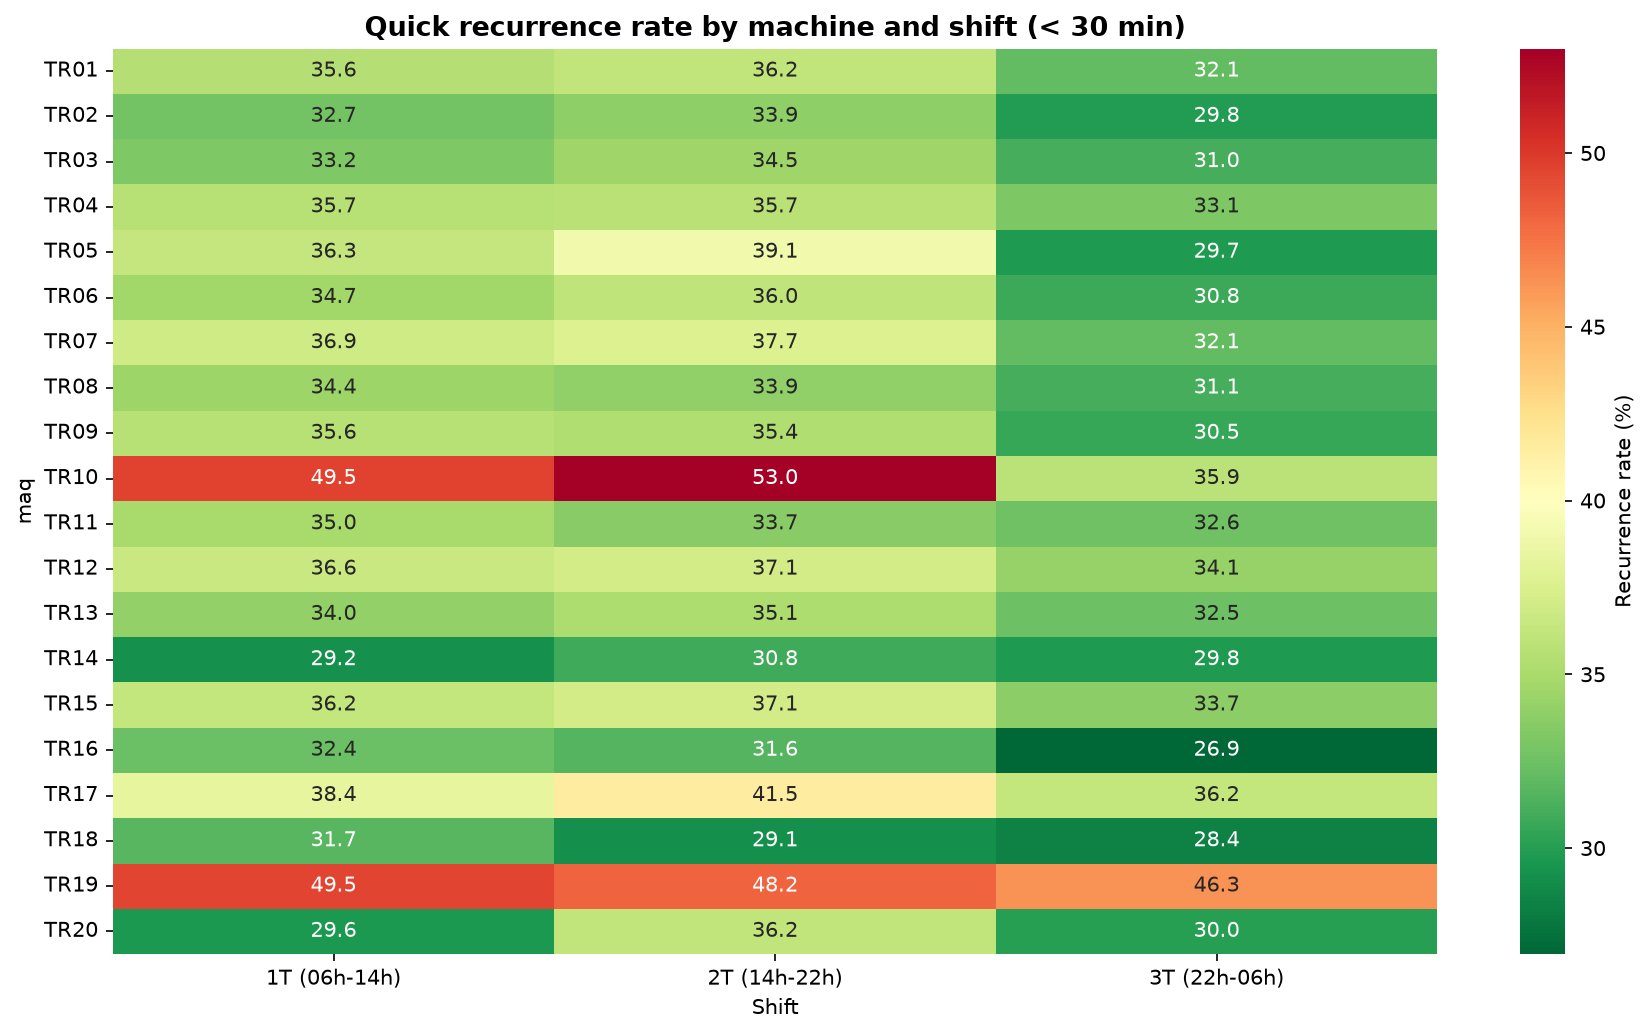
\includegraphics[width=0.6\linewidth]{recurrence_by_shift_30min_raw.png}
    \caption{Recorrências com IAT inferior a 30 minutos por máquina e turno de produção, calculadas sobre os eventos tratados em granularidade original.}
    \label{fig:recurrence-shift}
\end{figure}

Esses achados sustentam o uso do IAT como base de uma \textit{proxy} quantitativa de regimes em cascata, mas não comprovam propagação causal entre componentes. Para a modelagem, a intensidade diária do fenômeno será definida pelo número de eventos cujo IAT seja positivo e inferior a 30 minutos, atribuindo-se cada recorrência ao dia do alarme subsequente.

\subsection{Análise Espectral via Transformada de Fourier}

A análise espectral foi aplicada à série diária para identificar periodicidades que não são facilmente separáveis por inspeção visual. Antes da Transformada Rápida de Fourier (FFT), a série foi reindexada em frequência diária, os dias de contagem zero foram interpolados apenas para a estimação espectral e removeu-se a tendência linear. A potência das frequências positivas foi então convertida em função do período, em dias, e agrupada em faixas interpretáveis. O procedimento foi repetido na série bruta e na série sem outliers.

Na série bruta, a faixa de 2 a 4 dias concentrou 28,50\% da potência espectral, seguida pela faixa semanal, de 5 a 9 dias, com 17,38\%. As faixas quinzenal e mensal responderam por 7,05\% e 7,06\%, respectivamente. Componentes de 36 a 90 dias concentraram 8,65\%, enquanto as faixas trimestral, semestral, anual e plurianual reuniram 6,07\%, 3,65\%, 7,22\% e 7,70\%. Os picos de maior potência dentro das principais faixas ocorreram em aproximadamente 2,34, 7,97, 16,14 e 30,05 dias.

Após a remoção dos outliers, a participação da faixa de 2 a 4 dias diminuiu para 22,55\% e a semanal para 11,78\%. Essa redução mostra que os valores extremos amplificavam as oscilações rápidas, mas não as criavam, pois ambas permanecem relevantes na série tratada. Em contrapartida, aumentaram as participações relativas das faixas mensal (8,24\%), bimestral (11,96\%), trimestral (8,16\%) e plurianual (12,80\%). Como os percentuais são normalizados pela potência total, esses aumentos não significam necessariamente crescimento absoluto das componentes longas; parte do efeito decorre da perda de potência nas frequências curtas.

As participações quinzenal e anual permaneceram praticamente constantes, em torno de 7\%. Entretanto, somente a faixa anual preservou também o mesmo pico estimado, em 325,5 dias; o pico da faixa quinzenal deslocou-se de 16,14 para 10,17 dias. Os ciclos longos devem ser interpretados com cautela, pois a série contém poucos ciclos anuais completos, tendência estrutural, anos parciais e hiatos extensos. Em conjunto com as análises de sazonalidade e autocorrelação, a FFT oferece suporte mais robusto à persistência de padrões de curto prazo e de uma componente semanal.

Os espectros das duas versões da série são comparados na Figura~\ref{fig:fft-comparison}. A redução relativa da potência nas faixas mais curtas após o tratamento confirma a influência dos extremos, enquanto a permanência dos picos indica que os ciclos observados não são produzidos exclusivamente por eles.

\begin{figure}[H]
    \centering
    \begin{subfigure}{0.7\linewidth}
        \centering
        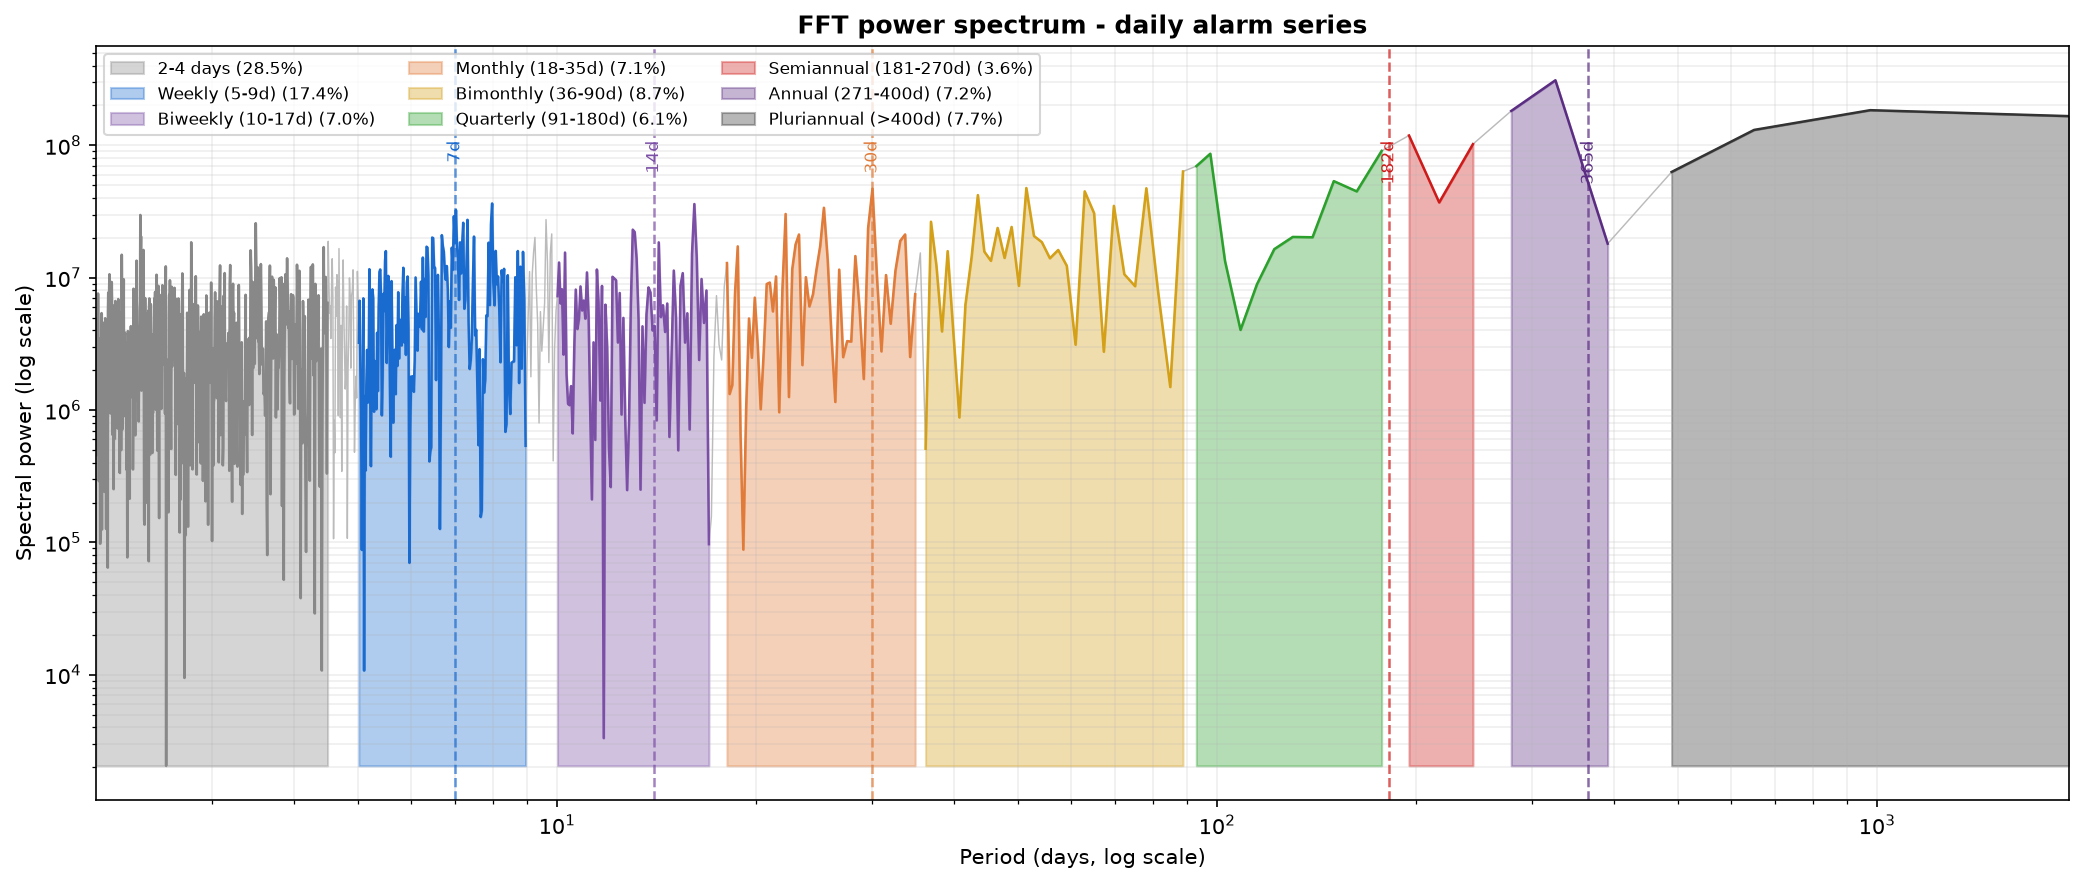
\includegraphics[width=0.7\linewidth]{fft_power_spectrum_raw.png}
        \caption{Espectro de potência da série bruta.}
        \label{fig:fft-raw}
    \end{subfigure}

    \vspace{0.4em}

    \begin{subfigure}{0.7\linewidth}
        \centering
        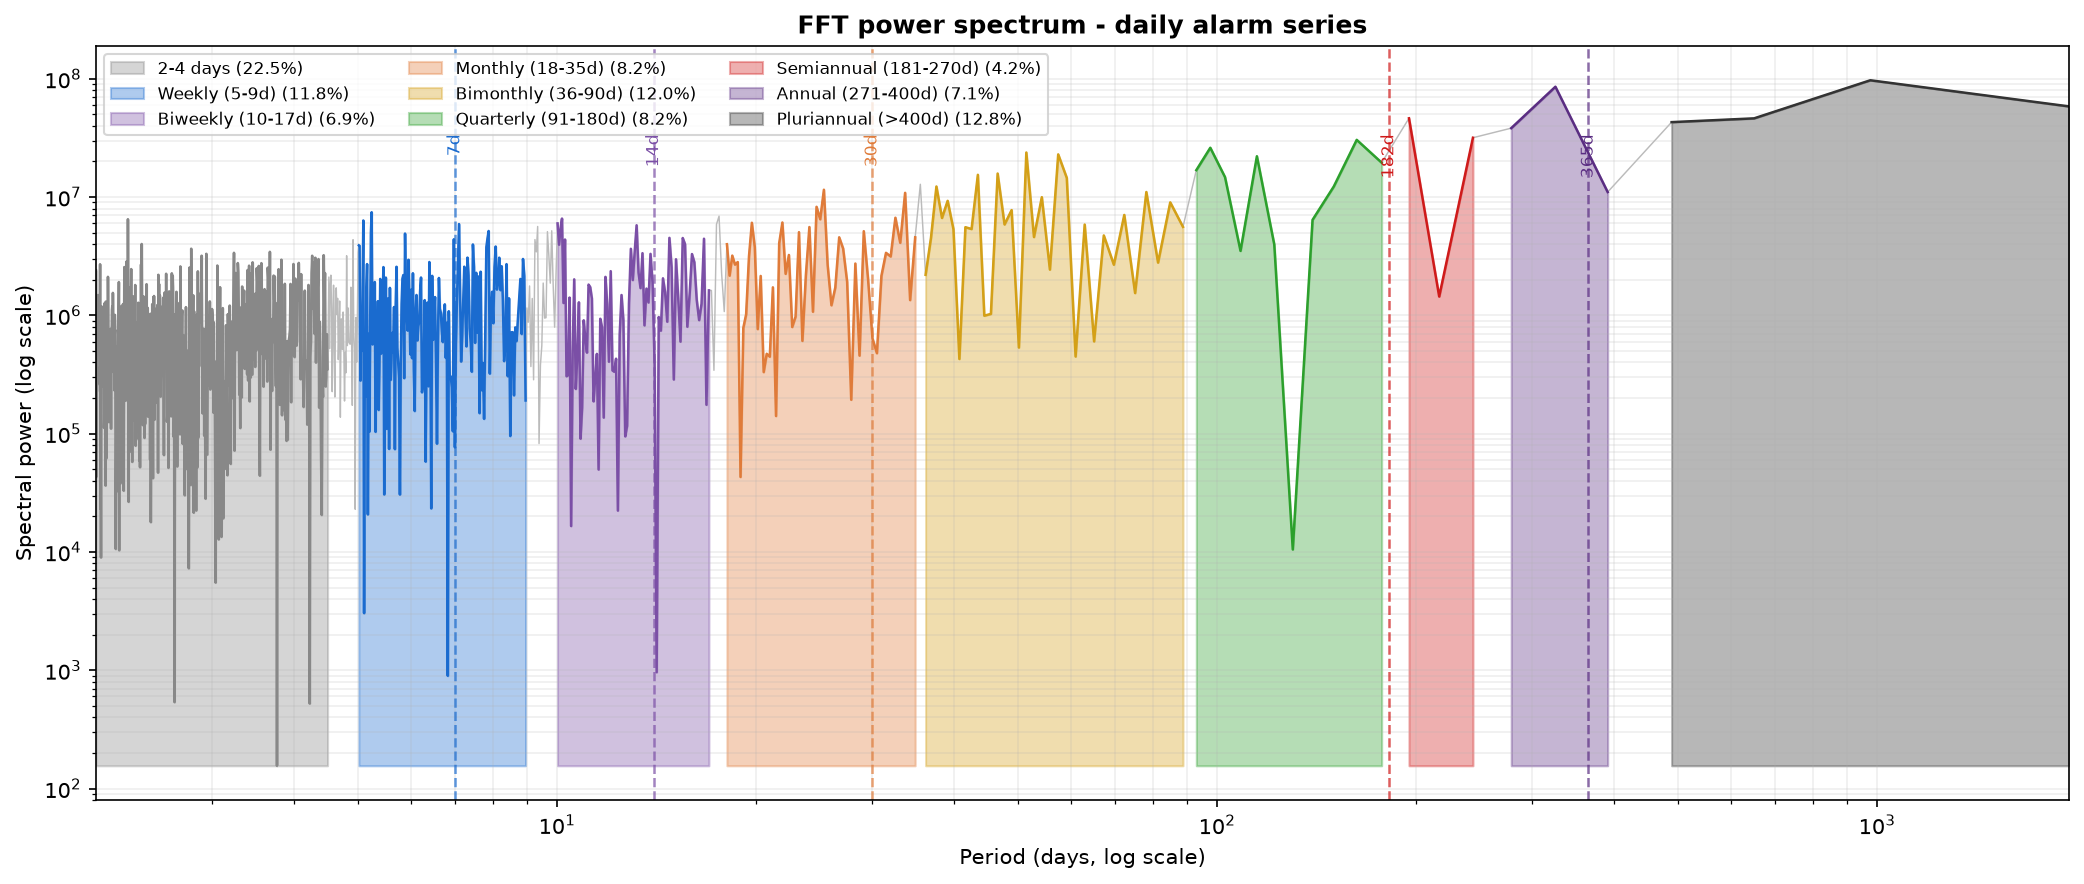
\includegraphics[width=0.7\linewidth]{fft_power_spectrum_no_outliers.png}
        \caption{Espectro de potência da série sem outliers.}
        \label{fig:fft-clean}
    \end{subfigure}
    \caption{Comparação dos espectros de potência da série diária. As faixas coloridas representam intervalos de periodicidade, e as linhas tracejadas marcam períodos de referência.}
    \label{fig:fft-comparison}
\end{figure}

\subsection{Decomposição Aditiva da Série Temporal}

A série diária também foi decomposta de forma aditiva em tendência, componente semanal, componente mensal e resíduo. A implementação emprega uma média móvel centrada de 30 dias para estimar a tendência; sobre a série sem tendência, calcula-se o efeito médio de cada dia da semana; e, após sua remoção, estima-se o efeito médio de cada mês. O resíduo corresponde à parcela não explicada por essas três componentes. O método é uma decomposição aditiva sequencial própria e não deve ser confundido com o algoritmo STL.

Na série bruta, a amplitude da tendência foi de 219,83 alarmes, a amplitude semanal de 13,36, a mensal de 6,60 e o desvio-padrão residual de 50,67. A presença de picos superiores a 600 e 800 alarmes por dia elevou a tendência local e concentrou grande parte da variação não explicada no resíduo. Ainda assim, a tendência revela mudanças persistentes: níveis mais elevados em partes de 2020 e 2021, oscilações durante 2022, forte redução em 2023 e recuperação a partir de 2024. Esses padrões descrevem o comportamento do registro de alarmes e não devem ser convertidos diretamente em afirmações sobre estabilidade da produção, para a qual não há medida de exposição disponível.

Na série sem outliers, a amplitude da tendência caiu para 100,21 alarmes, a semanal para 1,50, a mensal para 3,92 e o desvio-padrão residual para 24,72. A redução da amplitude semanal foi particularmente expressiva, confirmando que os valores extremos amplificavam o contraste entre dias da semana. A componente mensal apresentou maior estabilidade relativa, enquanto a forma geral da tendência foi preservada. Isso indica que as mudanças de longo prazo não eram produzidas exclusivamente pelos outliers, embora sua magnitude fosse substancialmente inflada por eles.

Os trechos de zero alarme permanecem visíveis como observações originais nos gráficos, mas são interpolados na série de trabalho utilizada para estimar as componentes. Assim, a tendência traçada dentro de um hiato representa uma continuidade estatística estimada, não atividade efetivamente observada. A decomposição é descritiva e utiliza informação de ambos os lados da janela centrada; suas componentes não devem ser inseridas diretamente como \textit{features} preditivas sem uma reformulação causal.

A Figura~\ref{fig:additive-decomposition-clean} apresenta a decomposição da série sem outliers. A escala reduzida permite observar com maior clareza a tendência de longo prazo, enquanto as componentes semanal e mensal permanecem pequenas diante da variação residual.

\begin{figure}[H]
    \centering
    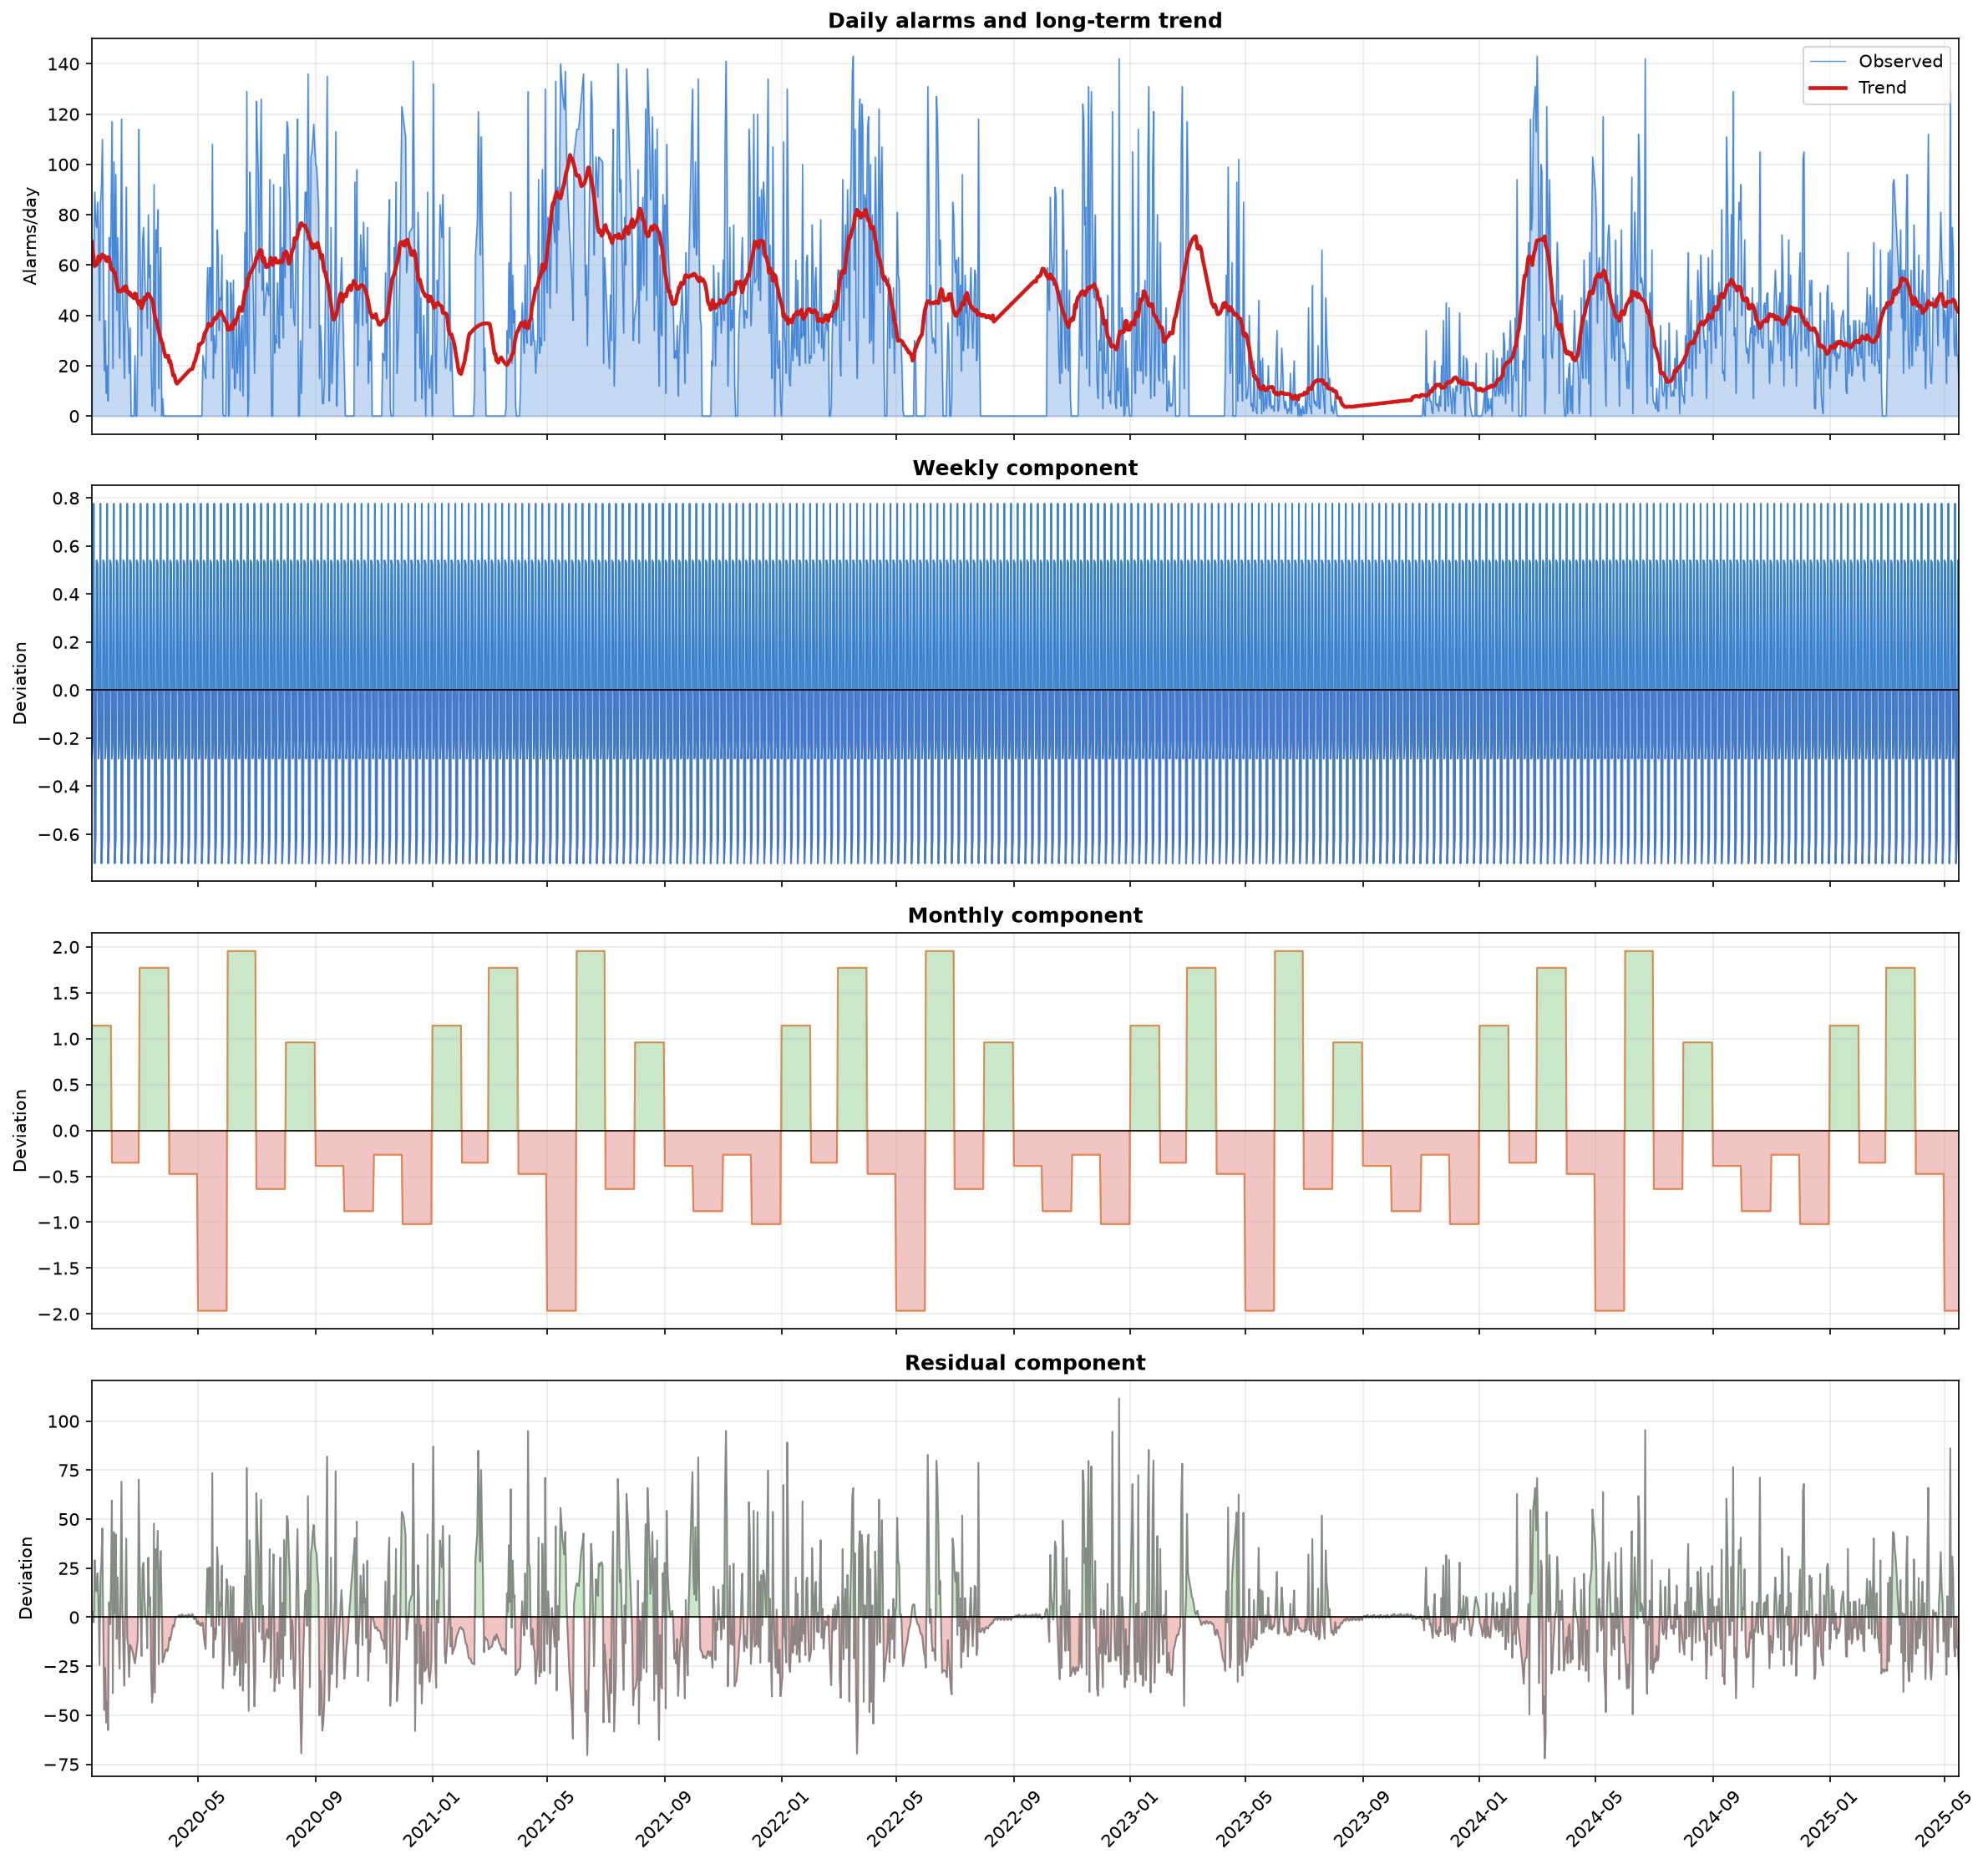
\includegraphics[width=0.6\linewidth]{additive_decomposition_no_outliers.png}
    \caption{Decomposição aditiva da série diária sem outliers em tendência, componente semanal, componente mensal e resíduo. Os valores dentro dos hiatos correspondem à continuidade estatística estimada para a decomposição.}
    \label{fig:additive-decomposition-clean}
\end{figure}

\subsection{Anomalias Cíclicas}

A caracterização categórica mostrou que a distribuição de alarmes entre as 20 máquinas é relativamente dispersa. TR10 registrou o maior volume, com 6.379 eventos, seguida por TR17, com 5.527; ainda assim, nenhuma máquina domina individualmente o conjunto, e a análise de Pareto não revelou uma concentração comparável à regra clássica de 80/20. A diferença entre os extremos é relevante --- TR16 possui 1.639 alarmes ---, mas o fenômeno está distribuído por toda a linha. Entre os tratos, as categorias 26 e 18 se destacam com 15.962 e 13.160 eventos, volumes substancialmente superiores aos demais.

Os códigos de alarme são fortemente concentrados em zero: FC1 apresenta 78.155 registros iguais a zero, FC2 apresenta 85.134 e FC3 apresenta 45.888. FC1 e FC3 exibiram correlação numérica próxima de 1, enquanto FC2 apresentou associação próxima de zero com ambos. Essa correlação não implica igualdade literal --- FC1 e FC3 coincidem em 51,90\% das linhas --- e deve ser interpretada com cautela, pois os códigos são categorias representadas por números. A ausência de um dicionário operacional e de informação de severidade impede inferir que códigos iguais a zero correspondam a alarmes inexplicados ou menos críticos. Por essa razão e pela ausência de relevância adicional identificada nas análises realizadas, os códigos foram descartados da engenharia de \textit{features}, assim como os demais campos operacionais não selecionados.

A distribuição intradiária apresentou pico geral às 6h e maior concentração entre 6h e 16h. Esse comportamento coincide com o início do primeiro turno e a transição para o segundo, mas não permite concluir que o volume de produção seja máximo nesse intervalo, uma vez que a base não contém unidades produzidas nem horas efetivamente trabalhadas. O terceiro turno concentra menos eventos em termos absolutos. No mapa hora por dia da semana, o domingo apresenta elevações no início do primeiro turno e, com maior intensidade, na transição entre 15h e 16h.

Na série bruta, o domingo reuniu 15.339 alarmes, enquanto os demais dias variaram entre 11.845 e 12.617. Considerando apenas dias com atividade registrada, a média dominical foi de 73,00 alarmes, 15,14 acima da média global; nos outros dias, as médias ficaram entre 53,74 e 57,56. Após o tratamento dos outliers, as médias condicionais tornaram-se muito mais próximas: 46,98 aos domingos e entre 45,20 e 47,58 nos demais dias. Portanto, a anomalia dominical é real na série bruta, mas é produzida principalmente por episódios extremos e não constitui, isoladamente, uma sazonalidade semanal uniforme ao longo de todo o período.

A distribuição mensal bruta atingiu seu maior volume em junho e apresentou elevações adicionais em março, maio, julho e setembro. A análise sem outliers reduziu os contrastes, mas preservou uma componente mensal de menor amplitude, também observada na decomposição aditiva. Essas anomalias de calendário justificam o uso de variáveis temporais na modelagem, desde que sejam codificadas sem acesso a informações posteriores ao instante de previsão.

\subsection{Autocorrelação da Série Diária}

A função de autocorrelação (ACF) foi calculada até 90 dias nas séries bruta e sem outliers. Em ambas, os coeficientes são positivos e decaem lentamente, permanecendo acima do intervalo de confiança de 95\% em praticamente todos os lags avaliados. Esse comportamento evidencia memória temporal, mas também reflete tendência, mudanças de regime e longas sequências de zeros; portanto, a significância isolada das barras não implica que um modelo deva incorporar todas as 90 defasagens.

Na série bruta, a autocorrelação parcial (PACF) identificou efeitos diretos em lags curtos e em pontos específicos, incluindo 7, 14, 21, 27, 28 e 29 dias. Na série sem outliers, os lags 1 a 5, 7 e 14 permaneceram entre os sinais mais consistentes, enquanto efeitos mais longos se tornaram esparsos. A remoção dos extremos elevou a ACF global de curto prazo e tornou seu decaimento mais regular, comportamento esperado porque a interpolação suaviza transições entre dias vizinhos. Esse aumento não deve ser interpretado automaticamente como fortalecimento físico da dependência.

A análise anual revelou heterogeneidade temporal. Em 2021, a série bruta apresentou sinais semanais nos lags 7, 14, 21 e 28; em 2024, os lags 28 e 30 tornaram-se levemente negativos; e, em 2025, a autocorrelação bruta de um dia alcançou 0,675, mas caiu para 0,368 após a remoção dos outliers. Esse último resultado sugere que os extremos de 2025 estavam temporalmente agrupados. Como 2025 contém somente dados até maio, suas estimativas possuem menor comparabilidade com as dos anos completos. A divergência entre os perfis anuais sugere estrutura temporal não estacionária, hipótese que deverá ser examinada formalmente durante a modelagem e considerada na validação cronológica.

A comparação global das funções de autocorrelação aparece na Figura~\ref{fig:acf-comparison}. O decaimento mais regular da série tratada é compatível com a suavização introduzida pela interpolação, enquanto a persistência de coeficientes positivos em ambas as versões confirma a presença de memória temporal.

\begin{figure}[H]
    \centering
    \begin{subfigure}{0.7\linewidth}
        \centering
        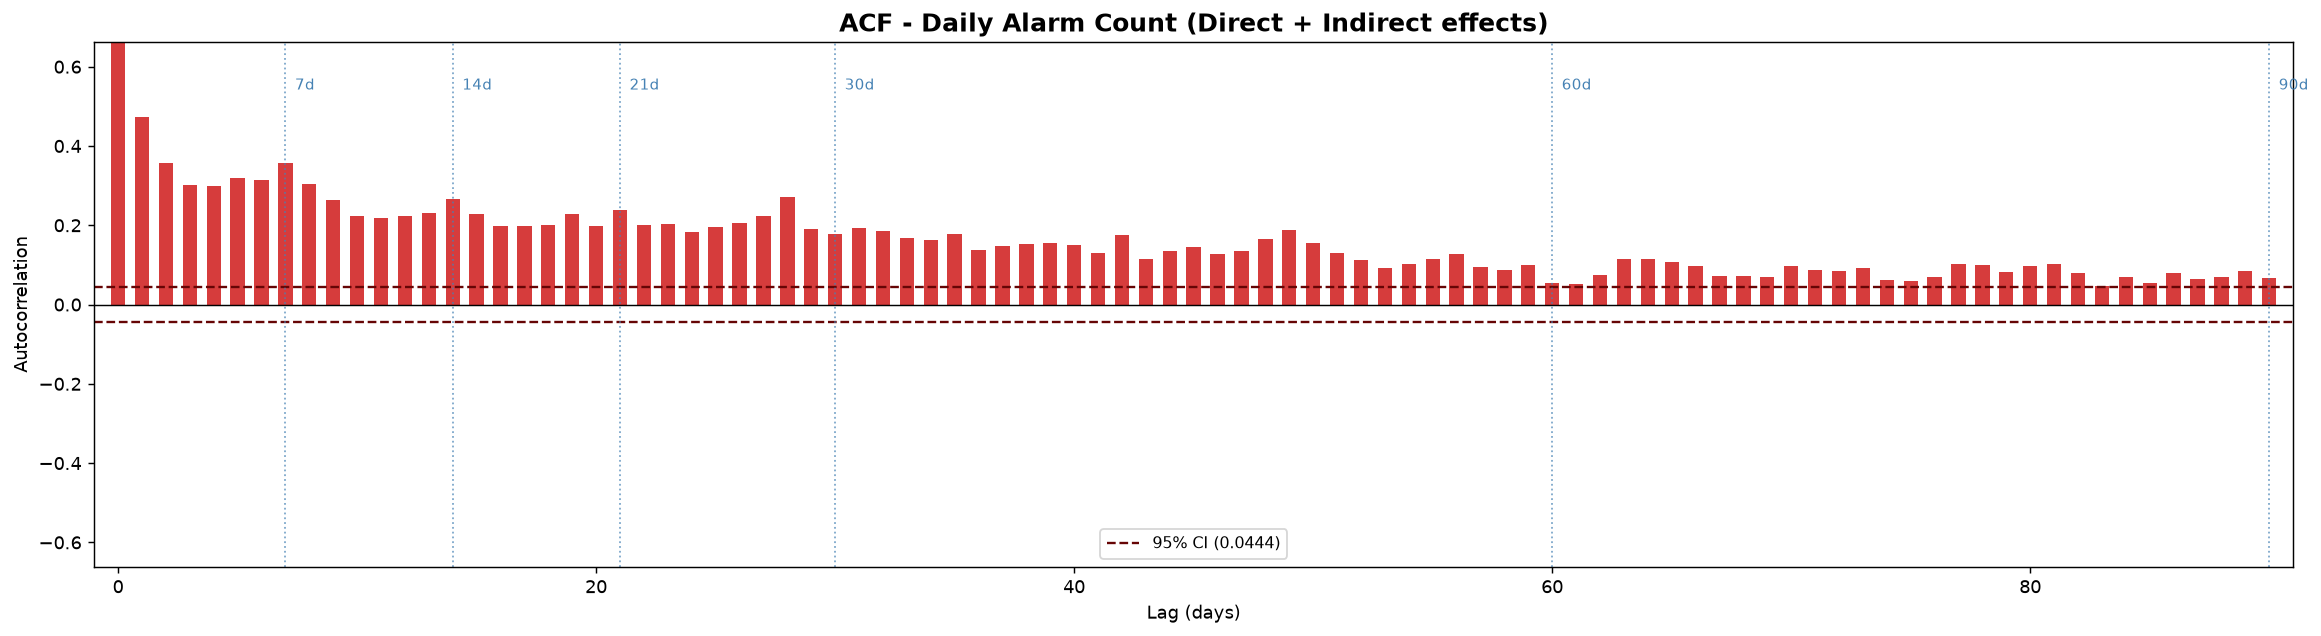
\includegraphics[width=0.7\linewidth]{acf_alarms_raw.png}
        \caption{ACF da série diária bruta.}
        \label{fig:acf-raw}
    \end{subfigure}

    \vspace{0.4em}

    \begin{subfigure}{0.7\linewidth}
        \centering
        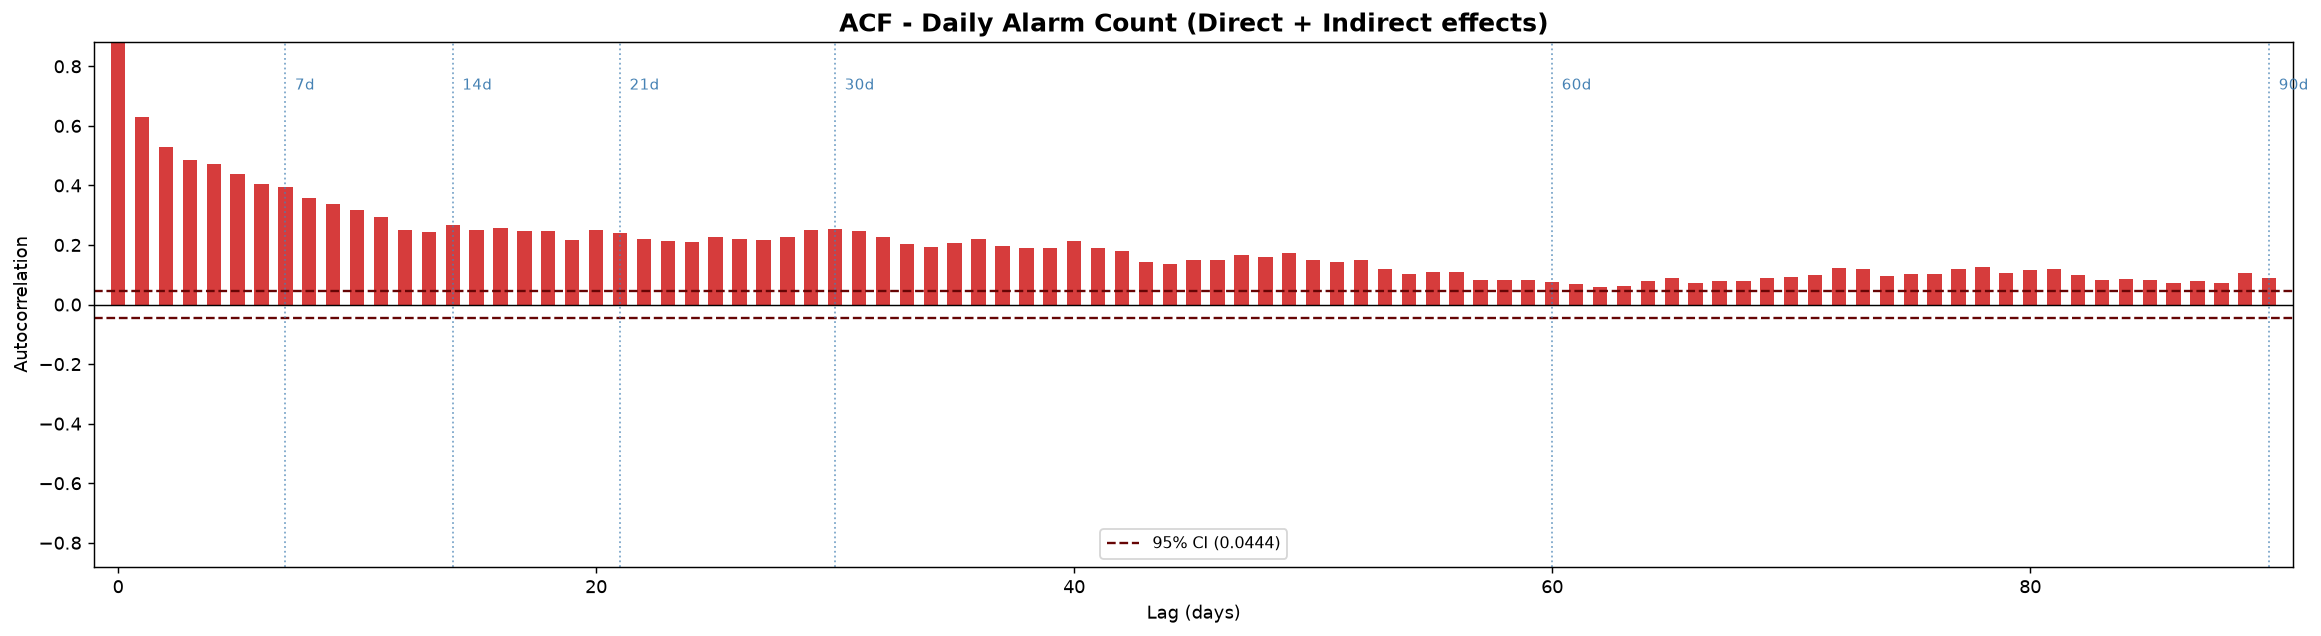
\includegraphics[width=0.8\linewidth]{acf_alarms_no_outliers.png}
        \caption{ACF da série diária sem outliers.}
        \label{fig:acf-clean}
    \end{subfigure}
    \caption{Função de autocorrelação da contagem diária de alarmes até 90 dias. As linhas tracejadas delimitam o intervalo de confiança de 95\%, e as linhas verticais marcam defasagens de referência.}
    \label{fig:acf-comparison}
\end{figure}

A instabilidade entre os anos, discutida acima, é detalhada na Figura~\ref{fig:acf-year-heatmap}. A divergência entre as linhas do mapa reforça que uma única estrutura de autocorrelação não descreve de forma uniforme todo o período observado.

\begin{figure}[H]
    \centering
    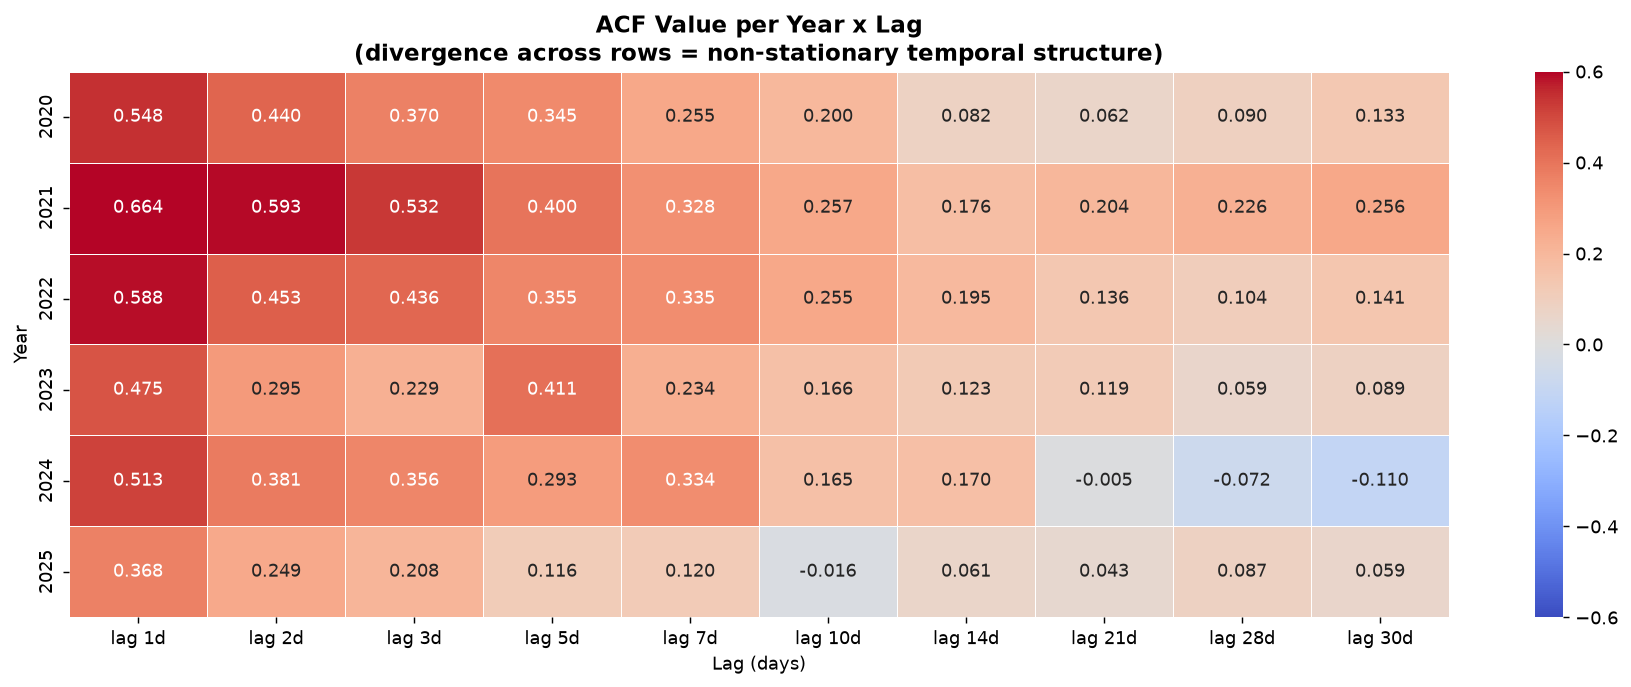
\includegraphics[width=0.7\linewidth]{acf_heatmap_year_lag_no_outliers.png}
    \caption{Coeficientes de autocorrelação por ano e defasagem na série sem outliers. A diferença entre os perfis anuais evidencia a não estacionariedade da estrutura temporal.}
    \label{fig:acf-year-heatmap}
\end{figure}

\subsection{Correlação Temporal com Variáveis Exógenas}

A associação entre o volume mensal de alarmes e as variáveis macroeconômicas foi avaliada com o coeficiente de Spearman, adequado a relações monotônicas sem pressupor normalidade. Foram consultadas as séries de Selic, IPCA de duráveis e balança comercial do Banco Central do Brasil e as Contas Nacionais Trimestrais do IBGE~\cite{bcb_selic_historico,bcb_ipca_duraveis,bcb_balanca_comercial,ibge_contas_nacionais_trimestrais}. As séries foram harmonizadas pela chave mensal \textit{AnoMes}. Como a fonte do PIB contém meses duplicados, seus coeficientes devem ser interpretados como exploratórios e com cautela adicional; a variável foi descartada da engenharia de \textit{features} final.

Na série bruta, a taxa Selic apresentou correlação de $-0{,}489$ com o volume mensal de alarmes (\textit{p} = 0,00005), o PIB apresentou $-0{,}359$ (\textit{p} = 0,00382), a balança comercial apresentou $-0{,}119$ (\textit{p} = 0,35232) e o IPCA de bens duráveis apresentou 0,434 (\textit{p} = 0,00038). Na série sem outliers, os coeficientes foram, respectivamente, $-0{,}410$ (\textit{p} = 0,00085), $-0{,}267$ (\textit{p} = 0,03438), $-0{,}075$ (\textit{p} = 0,56048) e 0,401 (\textit{p} = 0,00113). Selic e IPCA de bens duráveis preservaram direção, magnitude moderada e significância estatística nas duas versões; a balança comercial não apresentou evidência de associação; e o PIB, embora significativo, exibiu efeito mais fraco e sensível ao tratamento dos extremos.

Foram também avaliadas defasagens mensais entre $-3$ e $+3$ meses. Nenhuma variável apresentou ganho de associação suficientemente forte e estável que justificasse, apenas pela EDA, a seleção de múltiplos lags macroeconômicos. Esses resultados são associativos, não causais: tendências compartilhadas, paralisações e o pequeno número efetivo de meses podem gerar correlações espúrias. Para evitar vazamento temporal, qualquer variável exógena utilizada no modelo deverá ser associada à data em que se encontrava efetivamente disponível, e não simplesmente repetida em todos os dias do mês de referência.


\section{Engenharia de \textit{Features}}
\label{sec:features}

\subsection{Estratégia de Construção e Visão Geral}

A engenharia de \textit{features} foi redesenhada a partir do alvo de recorrência definido na EDA. Cada linha das matrizes representa o dia a ser previsto, enquanto toda variável operacional utiliza exclusivamente informação disponível até o término do dia anterior. Essa convenção impede que o volume ou as recorrências do próprio dia sejam utilizados para prever um alvo construído a partir dos mesmos eventos. As variáveis de calendário constituem a única exceção temporal, pois são conhecidas antecipadamente.

O \textit{pipeline} realiza uma única limpeza da base de eventos, calcula o IAT por máquina e constrói, no fuso horário local da planta, uma base diária intermediária com 1.953 datas. Nessa representação, 1.527 dias possuem ao menos um registro de alarme e 426 dias são marcados como potencial indisponibilidade. A diferença de um dia em relação à agregação exploratória em UTC --- 1.528 dias com registros e 425 dias de contagem zero --- decorre da conversão para \texttt{America/Recife} antes da atribuição de cada evento ao dia operacional. A aplicação do maior \textit{lag}, de 28 dias, e a exclusão conservadora dos dias sem registros resultam em 1.499 observações completas para modelagem.

Foram produzidos dois conjuntos finais, alinhados pelas mesmas datas e pelos mesmos valores do alvo:

\begin{table}[htbp]
    \centering
    \caption{Composição dos conjuntos finais de \textit{features}.}
    \label{tab:feature-sets}
    \begin{tabularx}{\textwidth}{lrrX}
        \hline
        \textbf{Conjunto} & \textbf{Observações} & \textbf{Preditores} & \textbf{Composição} \\
        \hline
        Simples & 1.499 & 16 & Calendário, histórico de \textit{gaps} e volume global de alarmes com defasagem \\
        Completo & 1.499 & 36 & Conjunto simples, Selic, IPCA de duráveis e volumes defasados de TR10, TR17 e TR19 \\
        \hline
    \end{tabularx}
\end{table}

O fluxo completo entre os eventos, a construção do alvo e os dois experimentos é resumido na Figura~\ref{fig:feature-pipeline}. A mesma base de 88.411 registros origina a contagem diária de recorrências, enquanto a distinção entre os modelos ocorre pela quantidade e pela natureza dos preditores disponíveis.

\begin{figure}[H]
    \centering
    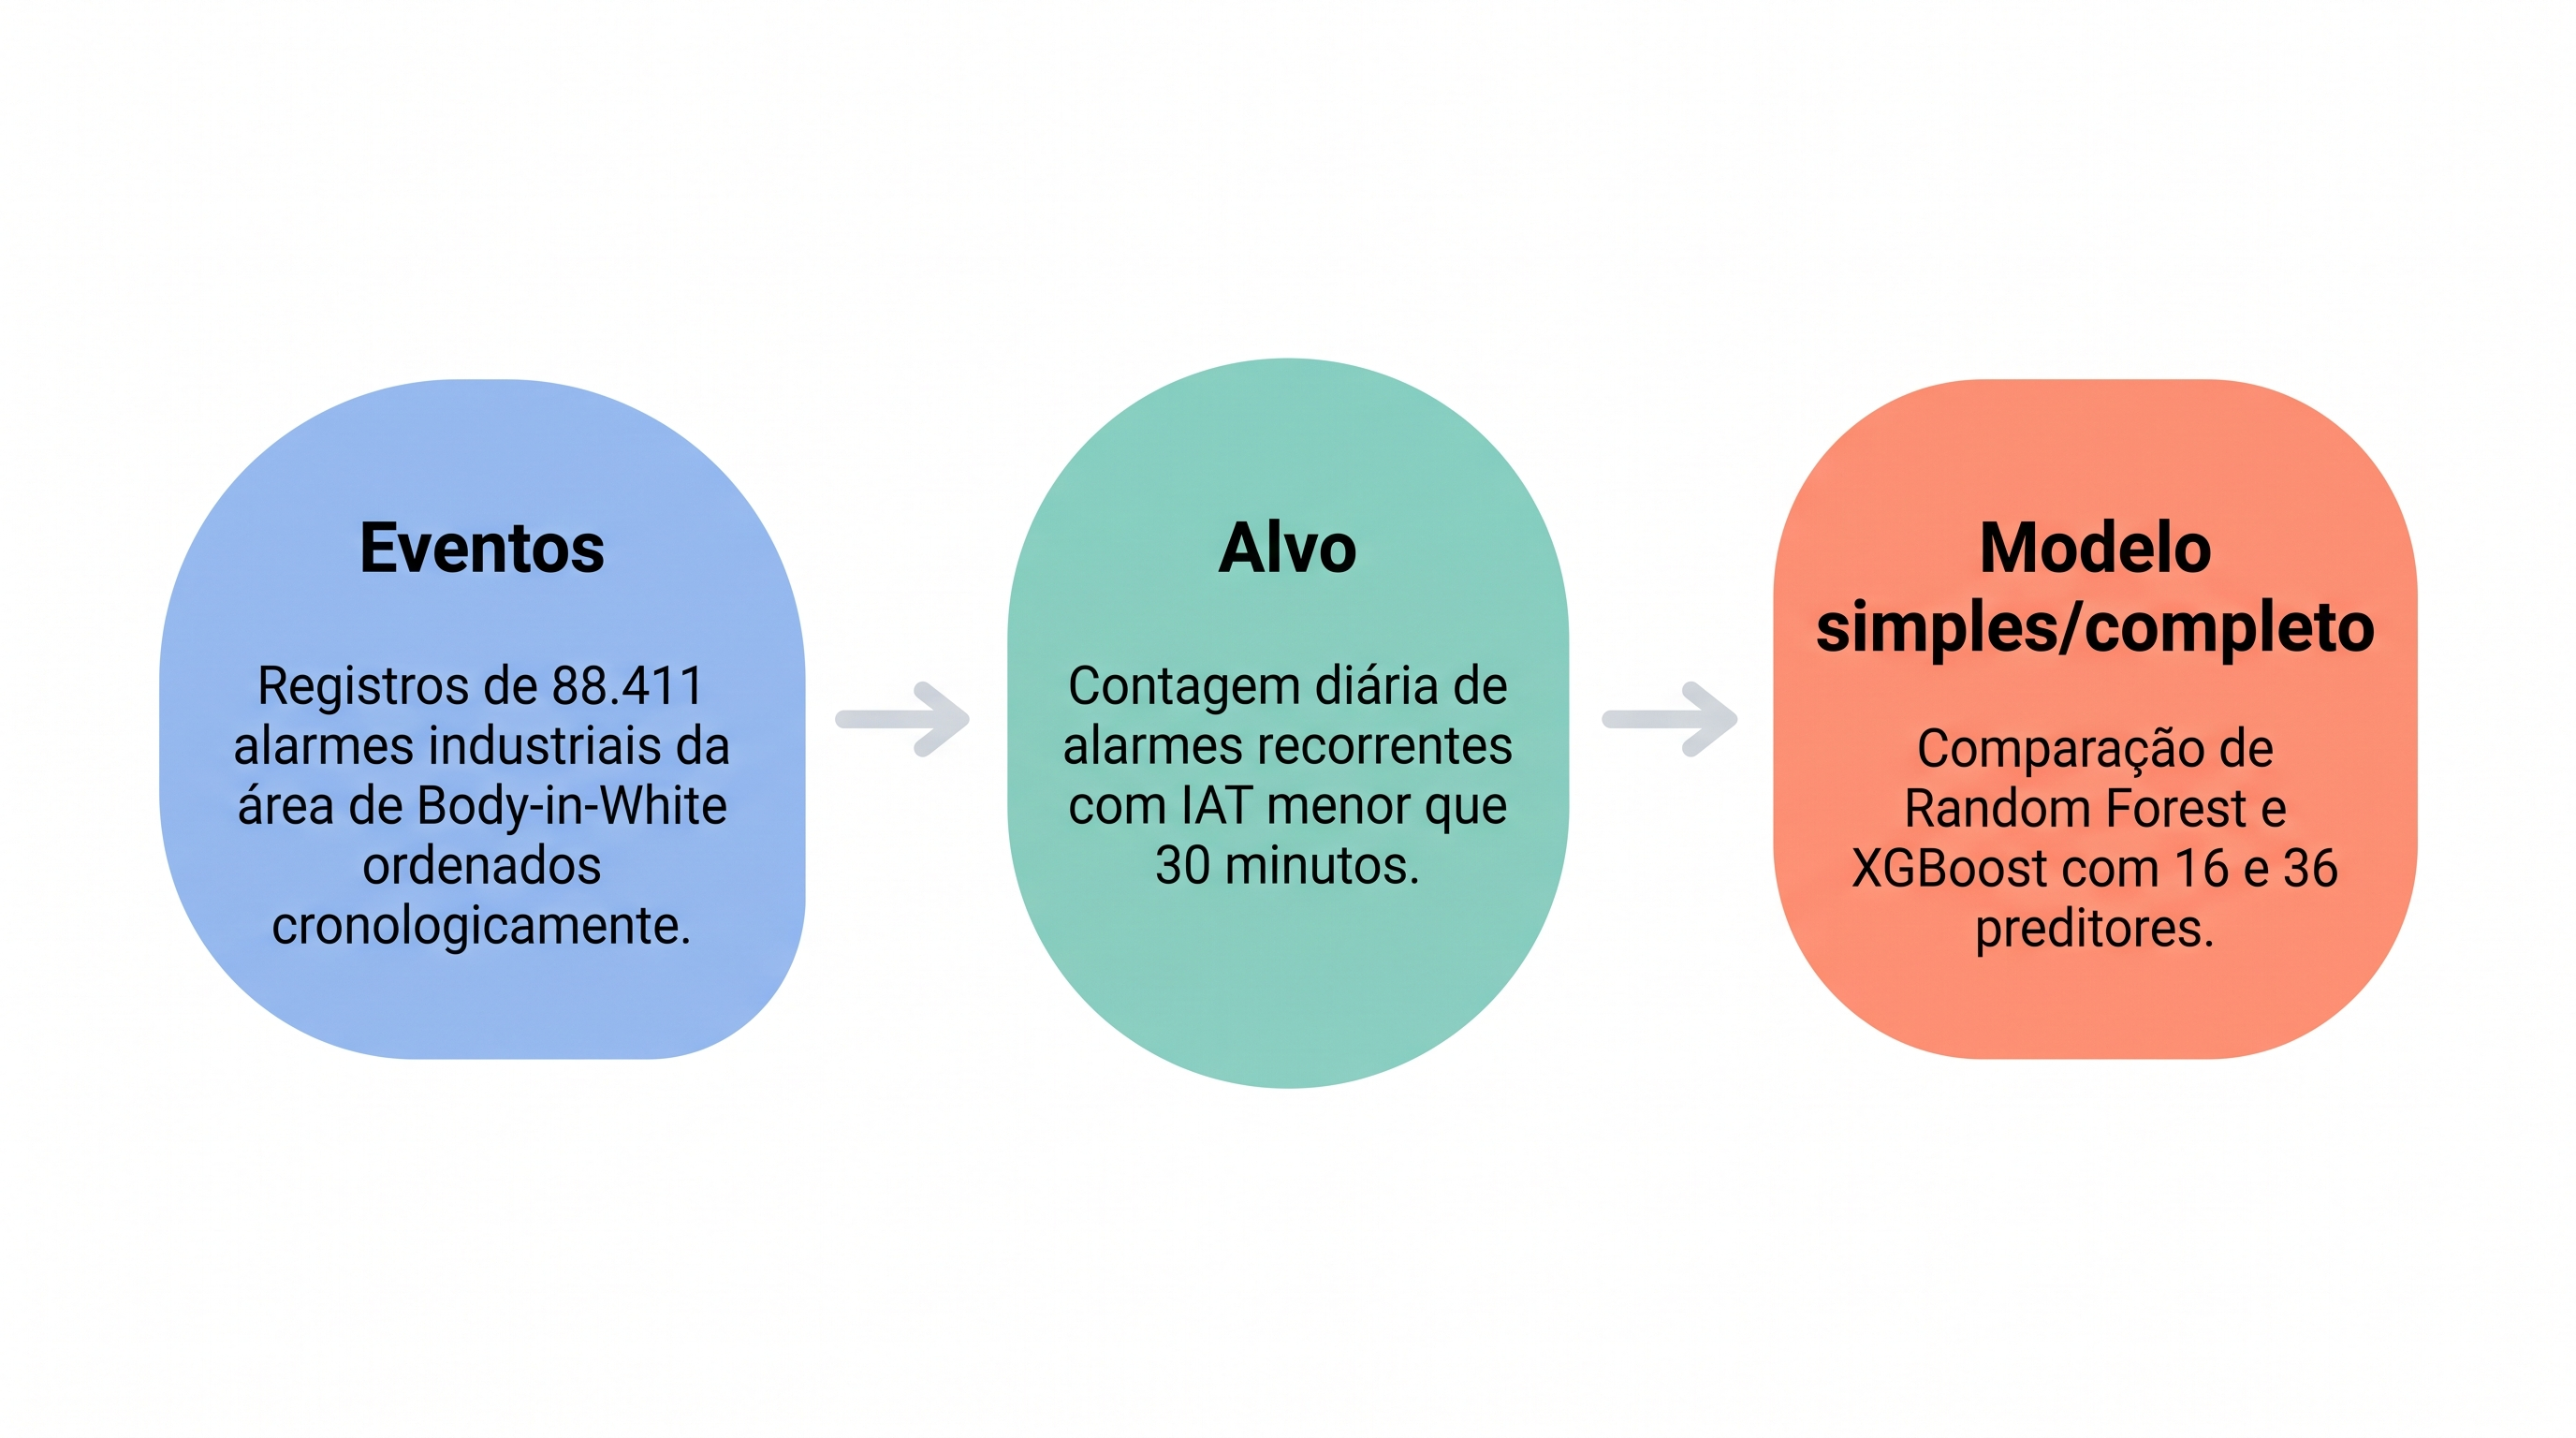
\includegraphics[width=0.7\linewidth]{diagrama_pipeline.jpg}
    \vspace{-1.5cm}
    \caption{Fluxo geral da preparação dos eventos, definição do alvo e comparação dos modelos simples e completo. O conjunto simples utiliza 16 preditores, e o completo utiliza 36.}
    \label{fig:feature-pipeline}
\end{figure}

Ambos preservam a data do alvo, a contagem \texttt{recurrences\_lt\_30m} e o metadado \texttt{target\_available}. As verificações finais confirmaram ordenação cronológica, unicidade das datas, alvo não negativo e ausência de valores ausentes entre os preditores das linhas elegíveis. Também foi verificado que o conjunto simples não contém variáveis específicas de máquina, enquanto o completo contém os seis \textit{lags} previstos para cada uma das três máquinas selecionadas.

\subsection{\textit{Features} Temporais e Cíclicas}

As variáveis de calendário são \textit{Year}, \textit{Month}, \textit{Day}, \textit{DayOfWeek}, \textit{WeekOfYear} e \textit{IsWeekend}. Elas descrevem a posição conhecida do dia-alvo no calendário e permitem que os modelos capturem mudanças graduais, padrões semanais, efeitos mensais e diferenças entre dias úteis e finais de semana. Embora a EDA tenha identificado anomalias em horários e transições de turno, a granularidade da modelagem é diária; por isso, a hora do evento e o turno não são empregados diretamente como atributos do dia.

\subsection{\textit{Features} de Janelas Deslizantes}

Médias móveis de três e sete dias foram consideradas em uma versão preliminar do \textit{pipeline}, mas não foram mantidas nos conjuntos finais. Além de introduzirem redundância com os volumes defasados, janelas que incluam o próprio dia produziriam vazamento do alvo. A versão final prioriza \textit{lags} pontuais, cuja origem temporal é explícita e auditável. Componentes da decomposição aditiva também não são utilizadas como \textit{features}, pois foram estimadas com janela centrada e possuem finalidade exclusivamente descritiva na EDA.

\subsection{\textit{Features} de Volume com Defasagem}

O volume diário global de alarmes foi defasado em 1, 3, 7, 14, 21 e 28 dias. Os \textit{lags} de 1 e 3 dias representam a memória de curto prazo observada na ACF e na PACF; 7 e 14 dias capturam a estrutura semanal mais consistente; e 21 e 28 dias permitem avaliar persistências mensais aproximadas identificadas em anos específicos. Nenhum volume do próprio dia-alvo é incluído. O \textit{pipeline} utiliza o volume bruto nos dias anteriores, preservando precisamente os episódios de alta atividade que podem anteceder recorrências, e não aplica interpolação futura ou limites calculados com observações posteriores ao corte de treino.

\subsection{\textit{Features} de Recorrências e Cascata}

O IAT é calculado após a ordenação cronológica dos eventos dentro de cada máquina. Para um evento $i$ da máquina $m$, define-se $IAT_{i,m}$ como a diferença, em minutos, entre seu instante e o alarme imediatamente anterior de $m$. O primeiro registro de cada máquina não possui IAT e não é contabilizado. A base completa contém 88.391 intervalos positivos válidos.

Uma recorrência rápida ocorre quando $0 < IAT_{i,m} < 30$ minutos. A agregação pelo dia do evento subsequente produziu 31.712 recorrências no período completo. Essa quantidade é utilizada como alvo, não como preditor contemporâneo. O desenho atual também não inclui \textit{lags} do próprio alvo, mantendo o modelo simples fundamentado em calendário, qualidade da continuidade e histórico de volume de alarmes. A eventual inclusão de recorrências passadas poderá ser avaliada posteriormente sem alterar a definição do alvo.

\subsection{\textit{Features} de Contexto de Hiatos}

Dias com contagem zero não são assumidos automaticamente como operação normal sem recorrências. Na base intermediária, esses dias recebem \texttt{target\_available = 0}; suas datas e volumes são preservados para manter a continuidade cronológica, mas eles são excluídos por padrão da matriz de treinamento. Trata-se de uma decisão conservadora diante da impossibilidade de separar, apenas pelos alarmes, ausência real de eventos, paralisação de planta e indisponibilidade de registros.

Quatro atributos causais transportam o contexto do \textit{gap} para os dias seguintes: \texttt{GapFlag\_lag1d}, indicador de que o dia anterior possui zero registros; \texttt{GapRunLength\_lag1d}, comprimento da sequência de zeros encerrada ou vigente no dia anterior; e \texttt{GapDays\_last7d} e \texttt{GapDays\_last30d}, números de dias sem registros nas janelas históricas correspondentes. Assim, o primeiro dia com atividade após os hiatos de 70 e 90 dias carrega explicitamente comprimentos 70 e 90, sem consultar datas posteriores ao alvo.

\subsection{\textit{Features} de Máquinas}

TR10 e TR17 foram selecionadas por apresentarem os maiores volumes globais de alarmes, enquanto TR19 foi selecionada por possuir o menor IAT mediano e a maior taxa de recorrência no limiar de 30 minutos. Para cada uma, o modelo completo incorpora o volume diário defasado em 1, 3, 7, 14, 21 e 28 dias. Os 18 atributos resultantes permitem representar concentrações localizadas de atividade sem usar o volume contemporâneo das máquinas, que seria parte direta da informação empregada na construção do alvo do próprio dia.

\subsection{Variáveis Exógenas Macroeconômicas}

O conjunto completo inclui exclusivamente Selic e IPCA de bens duráveis, variáveis que preservaram associações moderadas e estatisticamente significativas nas séries bruta e sem \textit{outliers}. Para representar disponibilidade realista, todos os dias de um mês recebem o valor do último mês concluído, com atraso mínimo de um mês. Valores ausentes nas bordas não são preenchidos a partir do futuro~\cite{bcb_selic_historico,bcb_ipca_duraveis}.

O PIB, obtido das Contas Nacionais Trimestrais do IBGE~\cite{ibge_contas_nacionais_trimestrais}, foi descartado porque apresentou associação mais fraca, sensível ao tratamento dos \textit{outliers} e sem ganho suficientemente claro para compensar sua baixa frequência temporal. A balança comercial do BCB~\cite{bcb_balanca_comercial} foi descartada por apresentar correlações fracas e não significativas nas duas séries. Os \textit{lags} macroeconômicos adicionais de $-3$ a $+3$ meses também não foram selecionados, pois a EDA não identificou melhora estável de associação. Essa seleção reduz a dimensionalidade e evita incorporar variáveis mensais com justificativa apenas circunstancial.

\section{Modelagem Preditiva}
\label{sec:modelagem}

\subsection{Definição do Alvo de Predição e Horizonte Temporal}

A variável-alvo é uma contagem diária não negativa. Para cada dia $d$, define-se:

\begin{equation}
    y_d = \sum_i \mathbb{1}\left(\operatorname{data}(i)=d \;\land\; 0 < IAT_i < 30\right),
    \label{eq:target}
\end{equation}

em que $i$ representa um evento de alarme, $IAT_i$ é o intervalo desde o alarme anterior da mesma máquina e $\mathbb{1}$ é a função indicadora. O horizonte adotado é de um dia: o modelo estima $y_d$ utilizando calendário conhecido e informações operacionais disponíveis até $d-1$. A tarefa é, portanto, de regressão de contagem. O alvo quantifica recorrência rápida e funciona como \textit{proxy} da intensidade de um regime de alarmes em cascata; não representa um rótulo externo de falha nem comprova propagação causal entre máquinas.

\subsection{Estratégia de Validação}

A avaliação foi dividida em duas etapas. Inicialmente, os últimos 365 dias de calendário foram isolados como teste final e permaneceram fora da seleção de algoritmos e hiperparâmetros. Esse período compreende 17 de maio de 2024 a 16 de maio de 2025 e contém 359 observações com alvo disponível. O período de desenvolvimento reúne 1.140 observações entre 8 de fevereiro de 2020 e 16 de maio de 2024.

Dentro do período de desenvolvimento, a validação utilizou janela expansiva com 730 dias iniciais de histórico, janelas nominais de validação de 180 dias e avanço de 180 dias. O procedimento produziu cinco \textit{folds}. Em cada iteração, todo o histórico anterior foi incorporado ao treinamento e a validação ocorreu exclusivamente em datas posteriores. Como dias sem alvo disponível foram excluídos, o número de observações por janela variou entre 79 e 138 e, em alguns \textit{folds}, a primeira data efetivamente avaliada foi posterior ao início nominal da janela.

Os dias marcados como indisponíveis e as primeiras linhas sem histórico completo de 28 dias não participam do ajuste nem da avaliação. Nenhum embaralhamento ou divisão aleatória é aplicado. Essa estratégia respeita a não estacionariedade identificada na ACF anual e mede a capacidade de generalização para regimes cronologicamente posteriores.

\subsection{Modelos, Configurações Experimentais e \textit{Baseline}}

Foram avaliados dois algoritmos de regressão baseados em árvores. O \textit{Random Forest Regressor} combina predições de múltiplas árvores construídas sobre amostras e subconjuntos de atributos, reduzindo a variância em relação a uma árvore individual~\cite{breiman2001randomforest,biau2012randomforests}. O \textit{XGBoost Regressor} constrói árvores sequencialmente e foi configurado com o objetivo \texttt{count:poisson}, coerente com a natureza não negativa da variável-alvo~\cite{chen2016xgboost}. As predições foram limitadas ao domínio não negativo e nenhuma normalização foi aplicada, pois os dois algoritmos não dependem de escala uniforme entre os preditores.

Cada algoritmo foi treinado com os conjuntos simples e completo, formando quatro experimentos: Random Forest simples, Random Forest completo, XGBoost simples e XGBoost completo. Para cada combinação foram avaliadas seis configurações compactas de hiperparâmetros. A seleção utilizou exclusivamente o menor MAE médio nos cinco \textit{folds} expansivos; o RMSE foi empregado como primeiro critério de desempate. Todos os ajustes utilizaram semente aleatória 42.

Como referência, foi implementado um \textit{baseline} de persistência que utiliza a quantidade de recorrências observada no dia civil anterior. O cálculo só é possível quando o alvo desse dia anterior está disponível; por isso, sua cobertura no teste final foi de 357 das 359 observações, ou 99,4\%. Essa diferença de cobertura foi mantida explícita na comparação.

As métricas selecionadas foram MAE, RMSE, coeficiente de determinação ($R^2$) e desvio médio de Poisson. O MAE foi adotado como critério principal por fornecer o erro médio diretamente em número de recorrências. O RMSE atribui peso maior aos erros extremos; o $R^2$ compara a capacidade explicativa com a predição pela média; e o desvio de Poisson complementa a avaliação da distribuição de contagens. O MAPE não foi utilizado porque o alvo contém valores zero.

\subsection{Resultados da Validação Expansiva}

As melhores configurações de cada experimento apresentaram os seguintes resultados médios no período de desenvolvimento:

\begin{table}[htbp]
    \centering
    \caption{Resultados médios da validação temporal expansiva.}
    \label{tab:expanding-validation}
    \begin{tabular}{llrrr}
        \hline
        \textbf{Algoritmo} & \textbf{Conjunto} & \textbf{MAE médio} & \textbf{DP do MAE} & \textbf{RMSE médio} \\
        \hline
        Random Forest & Simples & 17,000 & 4,905 & 27,925 \\
        Random Forest & Completo & 16,707 & 5,403 & 27,422 \\
        XGBoost & Simples & 13,943 & 4,849 & 26,848 \\
        XGBoost & Completo & \textbf{13,821} & \textbf{4,683} & \textbf{26,412} \\
        \hline
    \end{tabular}
\end{table}

O XGBoost completo obteve o menor MAE médio, mas sua vantagem sobre o XGBoost simples foi de apenas 0,122 recorrência, ou aproximadamente 0,9\%. Além disso, o modelo completo superou o simples em somente dois dos cinco \textit{folds}. As médias do alvo variaram de 1,76 a 20,77 recorrências entre as janelas, e o $R^2$ do XGBoost completo permaneceu negativo em todos os \textit{folds}. Esses resultados confirmam que o comportamento temporal é não estacionário e que a vantagem das variáveis adicionais não se mantém com a mesma intensidade em todos os regimes históricos.

As duas melhores configurações da busca do XGBoost completo também ficaram muito próximas: MAE médio de 13,821 para a configuração selecionada e 13,885 para a segunda colocada. Assim, não se observa um ótimo isolado fortemente definido dentro do espaço avaliado. A configuração escolhida possui 300 árvores, taxa de aprendizado de 0,05, profundidade máxima 6, peso mínimo de filho 1, amostragem de linhas e colunas de 0,8 e regularização L2 igual a 1.

\subsection{Desempenho no Teste Temporal Isolado}

Após a seleção dos hiperparâmetros, cada estimador foi reajustado utilizando as 1.140 observações do período de desenvolvimento e avaliado uma única vez nas 359 observações do teste final. Os resultados são apresentados na Tabela~\ref{tab:final-test}.

\begin{table}[htbp]
    \centering
    \caption{Desempenho no teste temporal isolado.}
    \label{tab:final-test}
    \resizebox{\textwidth}{!}{%
    \begin{tabular}{llrrrrrr}
        \hline
        \textbf{Modelo} & \textbf{Conjunto} & \textbf{Obs.} & \textbf{Cobertura} & \textbf{MAE} & \textbf{RMSE} & \textbf{$R^2$} & \textbf{Desvio de Poisson} \\
        \hline
        XGBoost & Completo & 359 & 100\% & \textbf{8,817} & \textbf{15,048} & \textbf{0,051} & \textbf{12,762} \\
        XGBoost & Simples & 359 & 100\% & 9,267 & 15,302 & 0,019 & 13,148 \\
        Random Forest & Simples & 359 & 100\% & 10,994 & 16,746 & $-0,175$ & 14,639 \\
        Random Forest & Completo & 359 & 100\% & 11,155 & 16,337 & $-0,118$ & 14,460 \\
        \textit{Baseline} lag-1 & Alvo anterior & 357 & 99,4\% & 11,462 & 20,425 & $-0,743$ & 62,747 \\
        \hline
    \end{tabular}}
\end{table}

O XGBoost completo apresentou o melhor valor em todas as métricas reportadas entre os modelos treinados. Em relação ao XGBoost simples, reduziu o MAE em 4,9\%, o RMSE em 1,7\% e o desvio de Poisson em 2,9\%. Na comparação restrita às 357 datas em que o \textit{baseline} estava disponível, o MAE do modelo vencedor foi 8,828, correspondente a uma redução de aproximadamente 23,0\% sobre a persistência diária. As duas configurações de Random Forest apresentaram $R^2$ negativo e tendência de superestimação da média: previram 13,85 e 14,39 recorrências por dia, respectivamente, diante de média observada de 10,80.

Apesar da primeira posição, o $R^2$ de 0,051 indica que o XGBoost completo explica apenas uma pequena parcela da variabilidade do período final. Sua superioridade deve ser interpretada como o melhor desempenho entre as alternativas avaliadas, e não como evidência de elevada precisão preditiva.

A evolução das previsões no teste final é apresentada na Figura~\ref{fig:xgboost-predictions}. A trajetória prevista acompanha parte das oscilações de baixa e média intensidade, mas permanece comprimida diante dos maiores valores observados, antecipando a limitação discutida na análise de erros.

\begin{figure}[H]
    \centering
    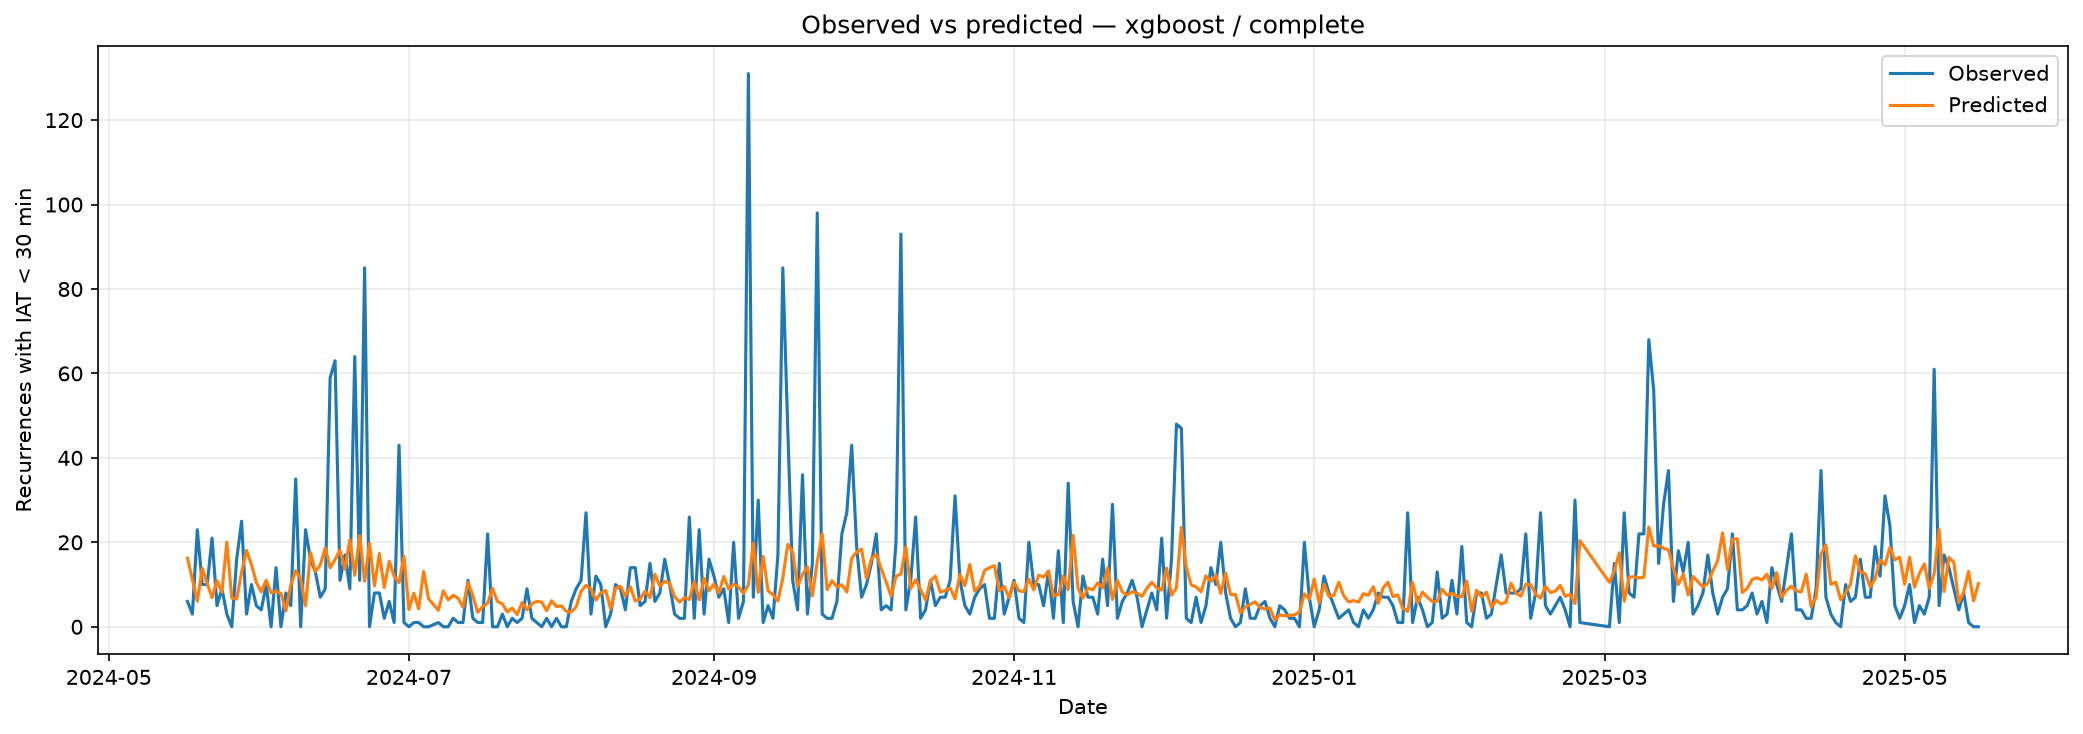
\includegraphics[width=0.7\linewidth]{xgboost_complete_predictions.png}
    \caption{Valores observados e previstos pelo XGBoost completo no teste temporal isolado, entre maio de 2024 e maio de 2025.}
    \label{fig:xgboost-predictions}
\end{figure}

\subsection{Importância das \textit{Features} no Modelo Vencedor}

A importância normalizada exposta pelo XGBoost completo foi agregada por grupo de variáveis:

\begin{table}[htbp]
    \centering
    \caption{Importância agregada das \textit{features} no XGBoost completo.}
    \label{tab:feature-importance}
    \begin{tabular}{lr}
        \hline
        \textbf{Grupo de \textit{features}} & \textbf{Importância agregada} \\
        \hline
        Volumes defasados de TR10, TR17 e TR19 & 48,8\% \\
        Indicadores de \textit{gaps} & 22,1\% \\
        Volume global de alarmes com defasagem & 19,0\% \\
        Variáveis de calendário & 5,8\% \\
        Selic e IPCA de duráveis & 4,3\% \\
        \hline
    \end{tabular}
\end{table}

Os volumes específicos das três máquinas concentraram quase metade da importância, com destaque para \texttt{TR19\_AlarmVolume\_lag1d}, segunda variável individual mais relevante, com 8,0\%. A primeira foi \texttt{GapFlag\_lag1d}, com 8,9\%, seguida por \texttt{GapDays\_last30d}, \texttt{AlarmVolume\_lag1d}, \texttt{AlarmVolume\_lag14d}, \texttt{GapDays\_last7d} e \texttt{TR10\_AlarmVolume\_lag1d}. A Selic respondeu por 2,7\% e o IPCA de duráveis por 1,5\%, reforçando que as variáveis macroeconômicas desempenharam papel secundário.

As variáveis acrescentadas pelo conjunto completo somaram 53,1\% da importância interna. Entretanto, essa proporção não deve ser interpretada como efeito causal nem como ganho preditivo de mesma magnitude: a redução do MAE em relação ao modelo simples foi de 4,9\% no teste e inferior a 1\% na média da validação expansiva. Parte da importância pode representar substituição ou redundância em relação ao volume global de alarmes.

A ordenação das variáveis individuais mais relevantes é mostrada na Figura~\ref{fig:xgboost-feature-importance}. O predomínio de indicadores de hiatos e de volumes recentes confirma que o contexto operacional próximo ao dia-alvo concentrou a maior parcela da importância interna do estimador.

\begin{figure}[H]
    \centering
    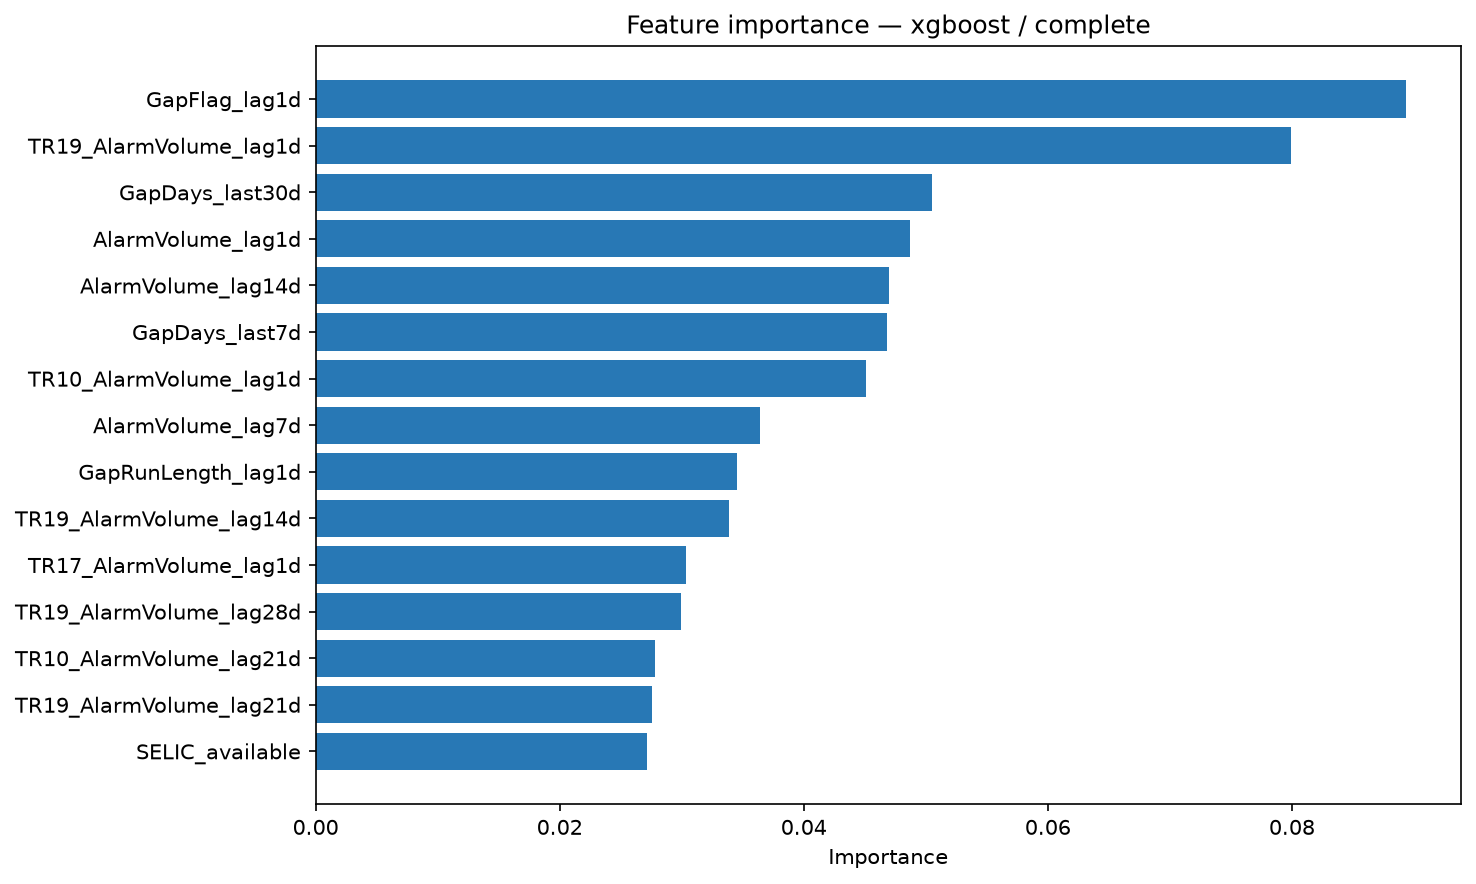
\includegraphics[width=0.6\linewidth]{xgboost_complete_feature_importance.png}
    \caption{Quinze maiores importâncias individuais do XGBoost completo. Os valores expressam a importância normalizada do estimador e não devem ser interpretados como efeitos causais.}
    \label{fig:xgboost-feature-importance}
\end{figure}

\subsection{Análise dos Erros e Limitações Preditivas}

No teste final, o alvo apresentou média de 10,80 e mediana de 6 recorrências, enquanto a média prevista foi de 10,04. A diferença média de 0,76 indica boa calibração agregada, com leve subestimação. Essa proximidade entre as médias, contudo, oculta uma forte compressão da amplitude: os valores observados variaram de 0 a 131, ao passo que as previsões ficaram entre 1,53 e 23,65. A correlação linear entre observado e previsto foi de apenas 0,236 e o erro absoluto mediano foi de 5,62 recorrências.

O modelo superestimou 237 dos 359 dias, principalmente aqueles com baixa atividade, e subestimou 122. Nos 32 dias com alvo zero, previu em média 7,44 recorrências. Por outro lado, os erros positivos pouco frequentes foram muito maiores: nos 38 dias com alvo entre 21 e 50, o MAE foi 18,11; nos 11 dias acima de 50, a média observada foi 78,45, a previsão média foi 14,33 e o MAE alcançou 64,12. No maior pico, de 131 recorrências em 8 de setembro de 2024, a previsão foi 9,93.

A comparação pareada com o XGBoost simples mostra que o completo foi melhor em 180 dias e pior em 179. O ganho concentrou-se nas faixas mais frequentes entre 1 e 20 recorrências; para alvos acima de 20, o conjunto completo apresentou erro médio ligeiramente maior. Portanto, as novas variáveis melhoraram o desempenho global sobretudo em dias de atividade baixa a moderada, sem resolver a antecipação de eventos extremos.

Os resíduos ainda apresentaram correlação de 0,224 na defasagem exata de sete dias e de 0,160 em quatorze dias, indicando que parte da estrutura semanal permaneceu sem representação adequada. Em conjunto com a variação acentuada entre \textit{folds}, esse resultado sugere que a principal limitação não é apenas algorítmica, mas também informacional: calendário, histórico de volumes, \textit{gaps}, máquinas selecionadas e variáveis macroeconômicas não são suficientes para caracterizar integralmente as mudanças de regime e os picos raros de recorrência.

A Figura~\ref{fig:xgboost-residuals} relaciona os resíduos às previsões do modelo vencedor. Os maiores resíduos positivos correspondem a picos observados que receberam previsões moderadas, enquanto a concentração de valores negativos em parte do domínio evidencia a superestimação frequente dos dias de baixa atividade.

\begin{figure}[H]
    \centering
    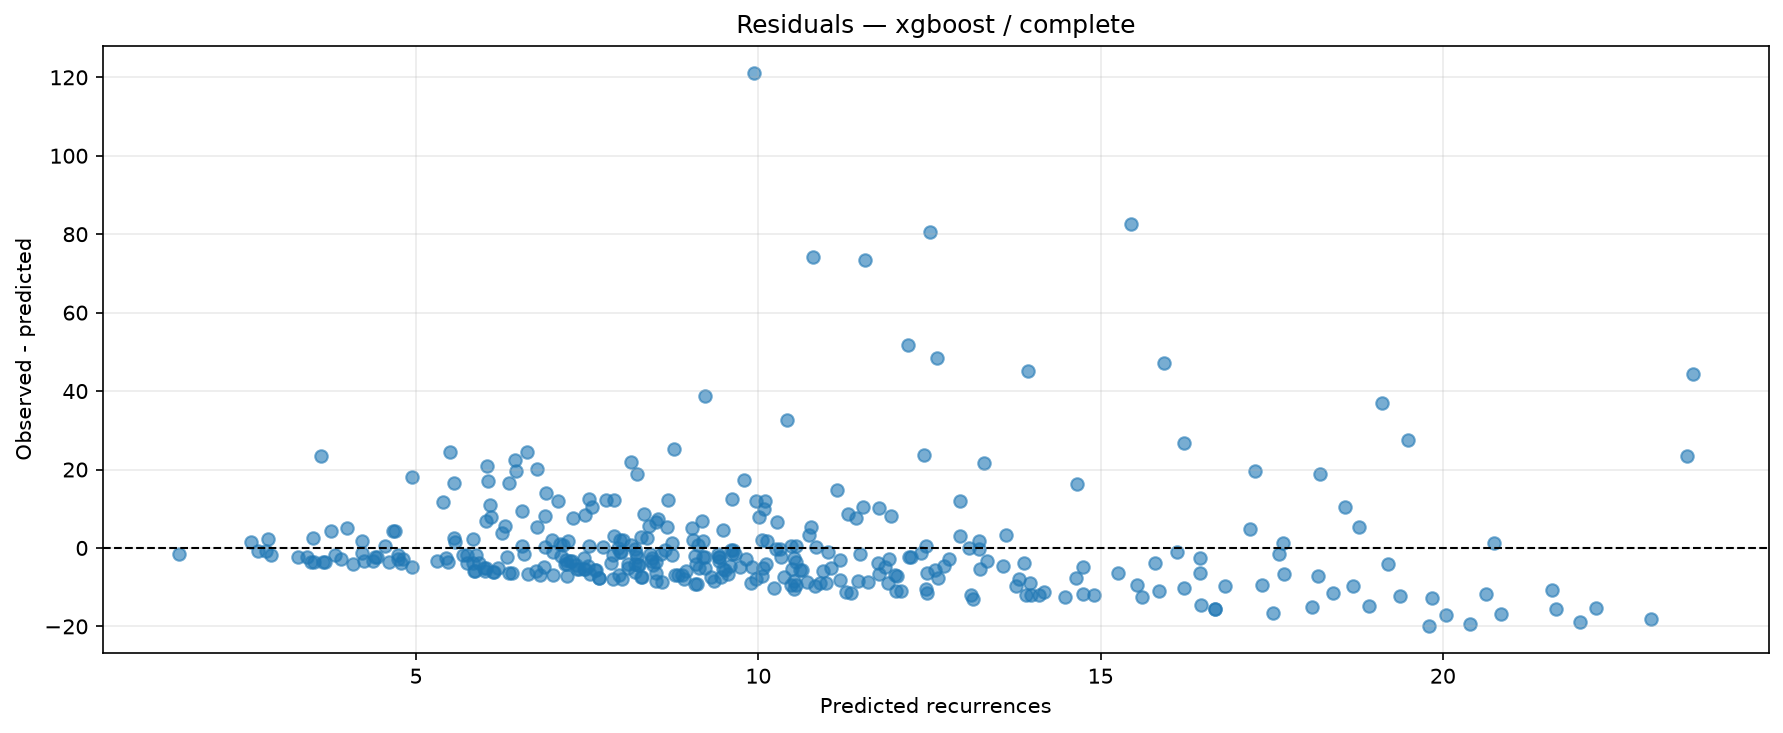
\includegraphics[width=0.7\linewidth]{xgboost_complete_residuals.png}
    \caption{Resíduos do XGBoost completo no teste final, definidos como valor observado menos valor previsto. A linha tracejada representa resíduo zero.}
    \label{fig:xgboost-residuals}
\end{figure}

Conclui-se que o XGBoost completo constitui o modelo final desta pesquisa por apresentar o menor MAE no teste temporal isolado e superar o \textit{baseline} e as demais combinações avaliadas. Seu uso deve, contudo, ser entendido como uma estimativa da intensidade cotidiana de recorrências, com capacidade limitada para antecipar picos extremos e com necessidade de recalibração diante de mudanças no regime operacional.
